\documentclass[]{article}
\usepackage{lmodern}
\usepackage{amssymb,amsmath}
\usepackage{ifxetex,ifluatex}
\usepackage{fixltx2e} % provides \textsubscript
\ifnum 0\ifxetex 1\fi\ifluatex 1\fi=0 % if pdftex
  \usepackage[T1]{fontenc}
  \usepackage[utf8]{inputenc}
\else % if luatex or xelatex
  \ifxetex
    \usepackage{mathspec}
  \else
    \usepackage{fontspec}
  \fi
  \defaultfontfeatures{Ligatures=TeX,Scale=MatchLowercase}
\fi
% use upquote if available, for straight quotes in verbatim environments
\IfFileExists{upquote.sty}{\usepackage{upquote}}{}
% use microtype if available
\IfFileExists{microtype.sty}{%
\usepackage{microtype}
\UseMicrotypeSet[protrusion]{basicmath} % disable protrusion for tt fonts
}{}
\usepackage[margin=1in]{geometry}
\usepackage{hyperref}
\hypersetup{unicode=true,
            pdfborder={0 0 0},
            breaklinks=true}
\urlstyle{same}  % don't use monospace font for urls
\usepackage{graphicx,grffile}
\makeatletter
\def\maxwidth{\ifdim\Gin@nat@width>\linewidth\linewidth\else\Gin@nat@width\fi}
\def\maxheight{\ifdim\Gin@nat@height>\textheight\textheight\else\Gin@nat@height\fi}
\makeatother
% Scale images if necessary, so that they will not overflow the page
% margins by default, and it is still possible to overwrite the defaults
% using explicit options in \includegraphics[width, height, ...]{}
\setkeys{Gin}{width=\maxwidth,height=\maxheight,keepaspectratio}
\IfFileExists{parskip.sty}{%
\usepackage{parskip}
}{% else
\setlength{\parindent}{0pt}
\setlength{\parskip}{6pt plus 2pt minus 1pt}
}
\setlength{\emergencystretch}{3em}  % prevent overfull lines
\providecommand{\tightlist}{%
  \setlength{\itemsep}{0pt}\setlength{\parskip}{0pt}}
\setcounter{secnumdepth}{0}
% Redefines (sub)paragraphs to behave more like sections
\ifx\paragraph\undefined\else
\let\oldparagraph\paragraph
\renewcommand{\paragraph}[1]{\oldparagraph{#1}\mbox{}}
\fi
\ifx\subparagraph\undefined\else
\let\oldsubparagraph\subparagraph
\renewcommand{\subparagraph}[1]{\oldsubparagraph{#1}\mbox{}}
\fi

%%% Use protect on footnotes to avoid problems with footnotes in titles
\let\rmarkdownfootnote\footnote%
\def\footnote{\protect\rmarkdownfootnote}

%%% Change title format to be more compact
\usepackage{titling}

% Create subtitle command for use in maketitle
\providecommand{\subtitle}[1]{
  \posttitle{
    \begin{center}\large#1\end{center}
    }
}

\setlength{\droptitle}{-2em}

  \title{}
    \pretitle{\vspace{\droptitle}}
  \posttitle{}
    \author{}
    \preauthor{}\postauthor{}
    \date{}
    \predate{}\postdate{}
  
\usepackage{booktabs}
\usepackage{longtable}
\usepackage{array}
\usepackage{multirow}
\usepackage{wrapfig}
\usepackage{float}
\usepackage{colortbl}
\usepackage{pdflscape}
\usepackage{tabu}
\usepackage{threeparttable}
\usepackage{threeparttablex}
\usepackage[normalem]{ulem}
\usepackage{makecell}
\usepackage{xcolor}

\begin{document}

title: ``R Notebook for Eel Habitat Map'' author: ``Nathaniel Legall''
output: html\_document

\begin{center}\rule{0.5\linewidth}{\linethickness}\end{center}

\textbf{Verion: 1.1}

\textbf{Date: 24/07/19 }

\textbf{Authored by: Nathaniel Legall}

\textbf{Checked by: }

This document has been written as technical guidance for the eel habitat
map produced as part of the Brue Valley Eel project.

\hypertarget{acknowledgements}{%
\section{Acknowledgements}\label{acknowledgements}}

We would like to thank the Somerset Internal Drainage Board for
providing the base structure data to produce the map. We are also
grateful to the Sustainable Eel Group got providing feedback on intitial
drafts of the map. This work was funded by the European Maritime
Fisheries Fund.

\hypertarget{executive-summary}{%
\section{Executive Summary}\label{executive-summary}}

\begin{center}\rule{0.5\linewidth}{\linethickness}\end{center}

\hypertarget{introduction}{%
\section{Introduction}\label{introduction}}

\hypertarget{eels-in-the-uk-and-somerset}{%
\section{Eels in the UK and
Somerset}\label{eels-in-the-uk-and-somerset}}

The European Eel (\emph{Anguilla anguilla}) is a long, narrow fish with
a complex lifecycle that encompasses living in both fresh and sea water.
Thought to spawn in the Sargasso Sea, European Eels enter the Brue
Valley via the Svern Estuary as glass eels. They then spend up to 20
years (possibly longer) in the valley's freshwater system before
migrating back out to sea to return to their spawning grounds. The
European Eel is currently classified as critically endangered.

\begin{figure}
\centering
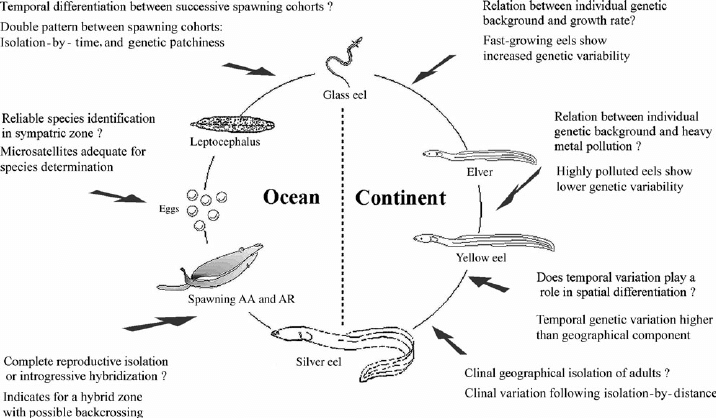
\includegraphics{Eel-life-cycle.png}
\caption{\textbf{Figure 1: The European Eel life cycle}}
\end{figure}

European Eel numbers have declined in Somerset, in line with national
trends, but they remain relatively common across the Levels. The local
rivers still support strong commercial fisheries.The River Brue runs
adjacent to the River Pattett which supports the second largest
commercial glass eel fishery in the UK. This is thought to be primarily
due to restricted access for eels into and within the catchment - due to
flood and water level sluices acting as barriers. The Somerset Wildlife
Trust nature reserves Catcott, Westhay Moor and Westhay Heath represent
excellent potential habitat to improve eel productivity. However, access
in and out is restricted due to blockages and sluices in, out and
between the wetlands, and to the waterways to the Brue.
\textless{}\textless{}\textless{}\textless{}\textless{}\textless{}\textless{}
HEAD =======

Diadromous species like Atlantic salmon (Salmo salar), European eel
(Anguilla anguilla) and migratory Brown trout (Salmo trutta, sea trout)
are particularly sensitive to barriers, as juvenile and adult life
stages must make extensive migrations across the freshwater environment
(e.g., Thorstad et al.~2010). Barriers placed lower in a river network
mostly affect diadromous fishes {[}Cote2009{]} {[}Fullerton2010{]}.
Barriers are therefore a potentially important constraint on production
and population persistence where access to and from spawning and rearing
habitats is limited (Holbrook, Kinnison \& Zydlewski 2011; Brown et
al.~2013), prevented (Gephard \& McMenemy 2004), or delayed (Venditti,
Rondorf \& Kraut 2000; Anon 2009; Nyqvist et al.~2017a)

\hypertarget{figure-2-comparison-of-european-eel-data-from-19-indicator-rivers-and-the-river-severn.-taken-from-pg.-66-of-our-nations-fisheries-environment-agency}{%
\section{\texorpdfstring{\protect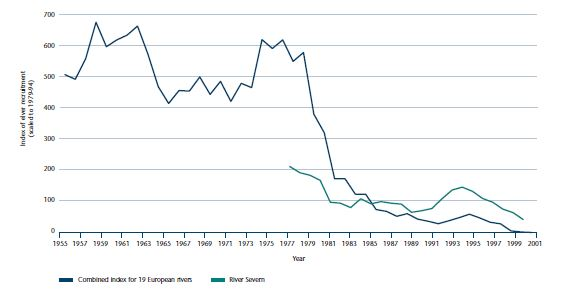
\includegraphics{Capture_OurNation'sFisheriespg.66.jpg}}{Figure 2: Comparison of European Eel data from 19 indicator rivers and the River Severn. Taken from pg. 66 of `Our Nation's Fisheries', Environment Agency}}\label{figure-2-comparison-of-european-eel-data-from-19-indicator-rivers-and-the-river-severn.-taken-from-pg.-66-of-our-nations-fisheries-environment-agency}}

\#Cultural value of European Eel in South West/Somerset? There is
evidence from the Domesday Book (Anon. 1086) of extensive eel fisheries
in the Thames, which persisted up until the end of the 19th century
{[}Defra2010{]}.
\textgreater{}\textgreater{}\textgreater{}\textgreater{}\textgreater{}\textgreater{}\textgreater{}
285b466eaaa74fa1a331da031f9b3b8ecc8d101f

Otter (\emph{Lutra lutra}) and mink (Mustela spp.) also take eel.
Although there is no available information on the likely levels of eel
predation by other species, {[}@Miranda2008{]} found that otter diet was
dominated by eel in the Somerset Levels, (28\% of the food biomass
annually and 56\% in Autumn). Despite this preference, populations of
these mammals are much lower than those of fish-eating birds and they
are likely to contribute a very small proportion of silver eel mortality
{[}@Defra2010{]}.

\hypertarget{economic-value-of-european-eel-in-south-westsomerset}{%
\section{Economic value of European Eel in South
West/Somerset}\label{economic-value-of-european-eel-in-south-westsomerset}}

There is evidence from the Domesday Book (Anon. 1086) of extensive eel
fisheries in the Thames, which persisted up until the end of the 19th
century {[}Defra2010{]}. Only hand-held dip nets are permitted for the
capture of glass eels or elvers, and fishing is concentrated where the
fish are plentiful and easy to catch -- principally in estuaries of the
Severn and other rivers draining into the Bristol Channel. The fishing
season is short, coinciding with the elvers entering rivers on spring
tides in April and May

Eels are caught commercially in a number of locations across England and
Wales, although East Anglia is the main centre. Adult eel are caught by
a variety of instruments including fyke nets, putcheons and weir traps.
A small amount of eel trawling also takes place off the south coast of
England and in the Thames Estuary. As with elvers, most adult eel
catches are exported; however, the main market for adult eels is
mainland Europe. Surprisingly, in the UK domestic market for jellying 90
per cent of the eels used come from farmed imports.

Fishing for eels in their various life stages can deliver significant
economic benefits to local rural economies. In 1997, the export value of
adult eels was estimated to peak at £2.5 million and, in 1998, that for
the elver or glass eel fishery was estimated at £2.6 million. While
small in comparison with the sums involved in the marine fish trade, eel
fisheries make a useful contribution to the UK's balance of payments.
The export value of elver fisheries peaked at £2.6 million in 1998, but
has since declined, with annual income per fisherman falling from £2000
to less than £900. As demand for elvers to stock eel farms has fallen,
so prices have also fallen, settling nearer to those of the late 1980s
and early 1990s. Adult eel exports now make only a very small
contribution to the balance of trade. The total first-sale value of the
adult eel fishery has declined from its peak of £2.5 million in the late
1990s to less than £0.5 million in 2000. Offset against this is the
import of between £170,000 (in 2000) and £380,000 (in 1999) of imported
fresh and frozen eels. The trend is one of falling demand for eels in
England and Wales and in mainland Europe. This is compounded by a
greater reliance on eel farming and cheaper imports from the Far East
depressing local prices.

\hypertarget{legal-requirements-to-protect-eels-in-somerset-uk}{%
\section{Legal requirements to protect Eels in Somerset \&
UK}\label{legal-requirements-to-protect-eels-in-somerset-uk}}

There is a legislative requirement to restore free passage, increase
habitat availability, and limit anthropogenic losses at intakes to aid
eel recovery and good ecological status; necessitating an improved
understanding of underlying processes {[}Piper2013a{]}. The Environment
Agency has a duty to maintain freshwater and Eel fisheries, both of
which play an important role in the wildlife interest of the Brue Valley
area. The fisheries are a major part of the wildlife interest especially
Eels which are widely distributed. Planned works to improve water level
management will have to consider fisheries improvements and any new
structures should allow for the free movement of Eels and Elvers
{[}@NA:18{]}. The EU regulation 1100/2007 -- article 2.4 states ``The
objective of each {[}EU{]} Eel Management Plan shall be to reduce
anthropogenic mortalities so as to permit with high probability the
escapement to the sea of at least 40 \% of the silver eel biomass
relative to the best estimate of escapement that would have existed if
no anthropogenic influences had impacted the stock''.
\textless{}\textless{}\textless{}\textless{}\textless{}\textless{}\textless{}
HEAD

For more informatin on the current conservation assessment of European
Eel please visit the
\href{https://www.iucnredlist.org/species/60344/45833138}{IUCN website}

=======

For more informatin on the current conservation assessment of European
Eel please visit the
\href{https://www.iucnredlist.org/species/60344/45833138}{IUCN website}
\textgreater{}\textgreater{}\textgreater{}\textgreater{}\textgreater{}\textgreater{}\textgreater{}
285b466eaaa74fa1a331da031f9b3b8ecc8d101f

\hypertarget{threats-to-european-eel-in-the-river-brue}{%
\section{Threats to European Eel in the River
Brue}\label{threats-to-european-eel-in-the-river-brue}}

It is important to recognise that a significant decline in eel
recruitment is in some way connected with a long-term change in oceanic
currents that can only be seen over decades. The parallel decline of the
recruitment of the American eel in some of its distribution area and the
correlation between the recruitment and the North Atlantic Oscillation
both tend to support this view.

Large-scale reductions of wetlands have resulted in a major loss of eel
habitat. Wetland loss - mainly caused by land reclamation for
agricultural use continues but at a much faster rate than before. The
Natural WET index - an indicator of change in area of all natural
wetlands shows a 30 per cent decline over the past 40 years. More recent
estimates from the IPBES show a 87 per cent loss of wetland habitat
globally in the last 300 years, and 54 per cent since 1900
{[}IPBES2019{]}. The reduction of wetland area directly affects European
Eel populations since they will face reduced habitat availability and
increased competition for food and other resources. All across Europe,
dams, weirs and dikes have been constructed in recent years (most of the
large dams have been built since the Second World War). These kinds of
barriers make it much more difficult (and in some cases quite
impossible) for eels to migrate up rivers; then, because their survival
in the lower reaches of rivers is density dependent, the number of adult
eels returning to sea is greatly reduced. Hydropower stations can kill
very many of the downstream migrating silver eels, and the available
information indicates a serious impact on the spawner population. The
turbine blades can kill anything from 10 per cent to 100 per cent for a
single passage, and the problem is inevitably compounded when there are
several turbines in series. It is estimated that between 2,500 and
10,000 tonnes of eels are killed each year in turbines -- the latter
figure being equal to the total declared commercial catch.

Another concern is that the accumulation of pollutants -- in particular
heavy metals and pesticides -- may impair the reproductive capability of
the eel. The emission of PCBs into the environment preceded the recent
decline of the European stock; and that PCBs and DDTs had a negative
impact on the lipid levels in eels. The review concluded that
contamination with PCBs and other pollutants may have contributed to the
decline of eel recruitment observed since 1980 {[}Defra2010{]}.

There is ample evidence that some fisheries can take so many eels that
they significantly reduce the number of potential spawners getting back
to sea. The available information also suggests that in extreme cases no
potential spawners may be reaching the sea.

\textless{}\textless{}\textless{}\textless{}\textless{}\textless{}\textless{}
HEAD Cormorants have been identified as the major eel predator. The food
intake of a cormorant is approximately 400 to 500 grams per day, and the
present estimate of the European breeding population is 250,000 to
300,000 pairs. Cormorants have been estimated to consume between 1800
tonnes of eels per year (two per cent of their yearly diet) and 9000
tonnes of eels per year (20 per cent of their yearly diet). =======
Cormorants have been identified as the major eel predator. The food
intake of a cormorant is approximately 400 to 500 grams per day, and the
present estimate of the European breeding population is 250,000 to
300,000 pairs. Cormorants have been estimated to consume between 1800
tonnes of eels per year (two per cent of diet throughout the whole year)
and 9000 tonnes of eels per year (20 per cent of diet through half of
the year).

The parasite Anguillicola crassus, introduced from the Far East, and
other pathogens can have an impact on eel populations. Anguillicola
crassus spread rapidly in theEuropean eel population in the early 1980s.
This parasite causes swim-bladder dysfunction and can impair the
migration of mature eels.
\textgreater{}\textgreater{}\textgreater{}\textgreater{}\textgreater{}\textgreater{}\textgreater{}
285b466eaaa74fa1a331da031f9b3b8ecc8d101f

The parasite \emph{Anguillicola crassus}, introduced from the Far East,
and other pathogens can have an impact on eel populations. Anguillicola
crassus spread rapidly in theEuropean eel population in the early 1980s.
This parasite causes swim-bladder dysfunction and can impair the
migration of mature eels.The decline of the eel in Europe is often
related to a reduction in the amount, quality and accessibility of its
continental habitat. One way through which habitat has been made more
accessible to European Eel aross the Brue and Parrett catchments has
been through the instllation of fish passes by the Environment Agency to
a number of medium sized (3 - 5 metres long) structures. The importance
of these aforementioned factors compared with the impact of exploitation
has not been quantified, but it seems likely that they are significant
in many European countries.

\hypertarget{head}{%
\section{\textless{}\textless{}\textless{}\textless{}\textless{}\textless{}\textless{}
HEAD}\label{head}}

The importance of these factors compared with the impact of exploitation
has not been quantified, but it seems likely that they are significant
in many European countries.

\hypertarget{rationale-for-project-work}{%
\section{Rationale for project work}\label{rationale-for-project-work}}

\begin{quote}
\begin{quote}
\begin{quote}
\begin{quote}
\begin{quote}
\begin{quote}
\begin{quote}
285b466eaaa74fa1a331da031f9b3b8ecc8d101f The River Brue catchment is
geographicaly adjacent to the River Parrett which supports the second
largest commercial glass eel fishery in the UK. The Brue is similar in
size to the Parrett catchment, yet it's eel populations and productivity
are believed to be much lower than the Parrett. This is thought to be
primarily due to restricted access for eels into and within the
catchment - due to flood and water level sluices acting as barriers.
Barriers represent one of the largest anthropogenic impacts on the
ecological status of rivers {[}Gido2015{]}, and they also potentially
restrict fishes' ability to respond to future environmental changes
{[}Cote2009{]}. Thus, river management aims to restore the longitudinal
connectivity of rivers to allow continuous migration and movement of
water, sediments and biotype {[}Radinger2018{]}. However, it is often
unclear whether the targeted barriers are also those most relevant for
fish species, particularly to track future habitat shifts caused by
environmental change The Somerset WIldlife Trust reserves at Catcott and
Westhay have excellent potential as eel habitat to improve eel
productivity. However, access in and out is restriced due to the
aforementioned blockages, out and between the wetlands, and to the
waterways to the Brue.
\end{quote}
\end{quote}
\end{quote}
\end{quote}
\end{quote}
\end{quote}
\end{quote}

This project will identify what future work can be undertaken to
maximise the eel productivity of the Brue Catchment.

\hypertarget{key-aims-of-project-work}{%
\subsection{Key aims of project work}\label{key-aims-of-project-work}}

The stated aims for this element of the funded project are as follows; -
To identify barriers to escapement and passageway through the lower Brue
catchment to the Severn Estuary
\textless{}\textless{}\textless{}\textless{}\textless{}\textless{}\textless{}
HEAD - To map a wetland ecological network that takes account of habitat
and permeability for eels \emph{this can be moved to the network
write-up} ======= - To map a wetland ecological network that takes
account of habitat and permeability for eels
\textgreater{}\textgreater{}\textgreater{}\textgreater{}\textgreater{}\textgreater{}\textgreater{}
285b466eaaa74fa1a331da031f9b3b8ecc8d101f

\hypertarget{methodology}{%
\section{Methodology}\label{methodology}}

\hypertarget{study-area}{%
\subsection{Study Area}\label{study-area}}

The Brue Valley is part of the Somerset Levels and Moors (a low-lying
region of north and central Somerset bisected by limestone ridges and
hills) and covers almost 12,500 hectares of the floodplain of the River
Brue between Glastonbury in the East and the M5 in the West. The
Somerset Levels and Moors is a landscape of highly artificial rivers and
intense human management of water and it is this intense management that
determines habitat type and land use in the Brue Valley. Habitats
present in the Brue Valley include; - Coastal and Floodplain Grazing
Marsh - Lowland Meadow - Purple moor grass - Rush pasture - Fen -
Reedbed - Wet Woodland
\textless{}\textless{}\textless{}\textless{}\textless{}\textless{}\textless{}
HEAD The Brue Valley is bisected by the North Drain, River Brue, South
Drain and Huntspill River.
\href{http://ea-lit.freshwaterlife.org/archive/ealit:950}{Gold Corner
pumping station} is at the junction of the South Drain, Cripps River and
the Huntspill River. The station is used to prevent flooding in the Brue
Valley, maintaining acceptable water levels in the South Drain and to
keep the Huntspill River - which acts as a local reservoir - topped up
during the Summer. Water is lifted some 3 metres (8.5 feet) from the
South Drain to the Huntspill River.

The Somerset Wildlife Trust's Catcott and Westhay nature reserves exist
in the centre of the Brue Valley. Catcott Nature Reserve (Centre grid
reference = ST404411) comprises a series of low-lying fields, carr and
former peat workings with numerous ditches that forms part of the
extensive grazing marsh and high level wet ditch system. Near the centre
is the original reserve known as Catcott Heath, a mosaic of widely
differing habitats -- most importantly NVC S24 fen vegetation, with milk
parsley (\emph{Puecedanum palustre}) and bog myrtle (\emph{Myrica
gale}), mixed broadleaf woodland, peat ponds and ditches. To the west is
a partially worked peat digging, known as Great Fen comprising reed fen
where the peat has been removed and restored fen where sufficient peat
remains. 1,000,000 glass eels were introduced to this compartment during
2015. Separate and to the south lies a small restored former peat
working, known as Catcott Fen, with a wet reed bed community. Westhay
Moor National Nature Reserve and Westhay Moor Nature Reserve comprise
areas of wetland mosaics including tall fen vegetation, marshy
grassland, willow scrub, alder carr, small ponds, open water channels
and the remnants of acid raised mire form previously used for peat
extraction in the heart of the peat moors on the Somerset Levels.
Catcott and Westhay Nature Reserves represent areas of optimal habitat
for European Eel of different life stages (West, 2019) so were used as
the targets during GIS (Geographic Information System) analysis.

\hypertarget{a-bounding-box-was-set-encompassing-the-majority-of-the-legacy-brue-valley-living-landscape-project-area.}{%
\section{A bounding box was set encompassing the majority of the legacy
Brue Valley Living Landscape project
area.}\label{a-bounding-box-was-set-encompassing-the-majority-of-the-legacy-brue-valley-living-landscape-project-area.}}

The Brue Valley is bisected by the North Drain, River Brue, South Drain
and Huntspill River.
\href{http://ea-lit.freshwaterlife.org/archive/ealit:950}{Gold Corner
pumping station} is at the junction of the South Drain, Cripps River and
the Huntspill River. The station is used to prevent flooding in the Brue
Valley, maintain acceptable water levels in the South Drain and to keep
the Huntspill River -which acts as a local reservoir - topped up during
the summer. Water is lifted some 3 metres (8.5 feet) from the South
Drain to the Huntspill River.

{[}How were the Catcott and Westhay reserves completed?{]} see Catcott
CMP
\textgreater{}\textgreater{}\textgreater{}\textgreater{}\textgreater{}\textgreater{}\textgreater{}
285b466eaaa74fa1a331da031f9b3b8ecc8d101f

\begin{figure}
\centering
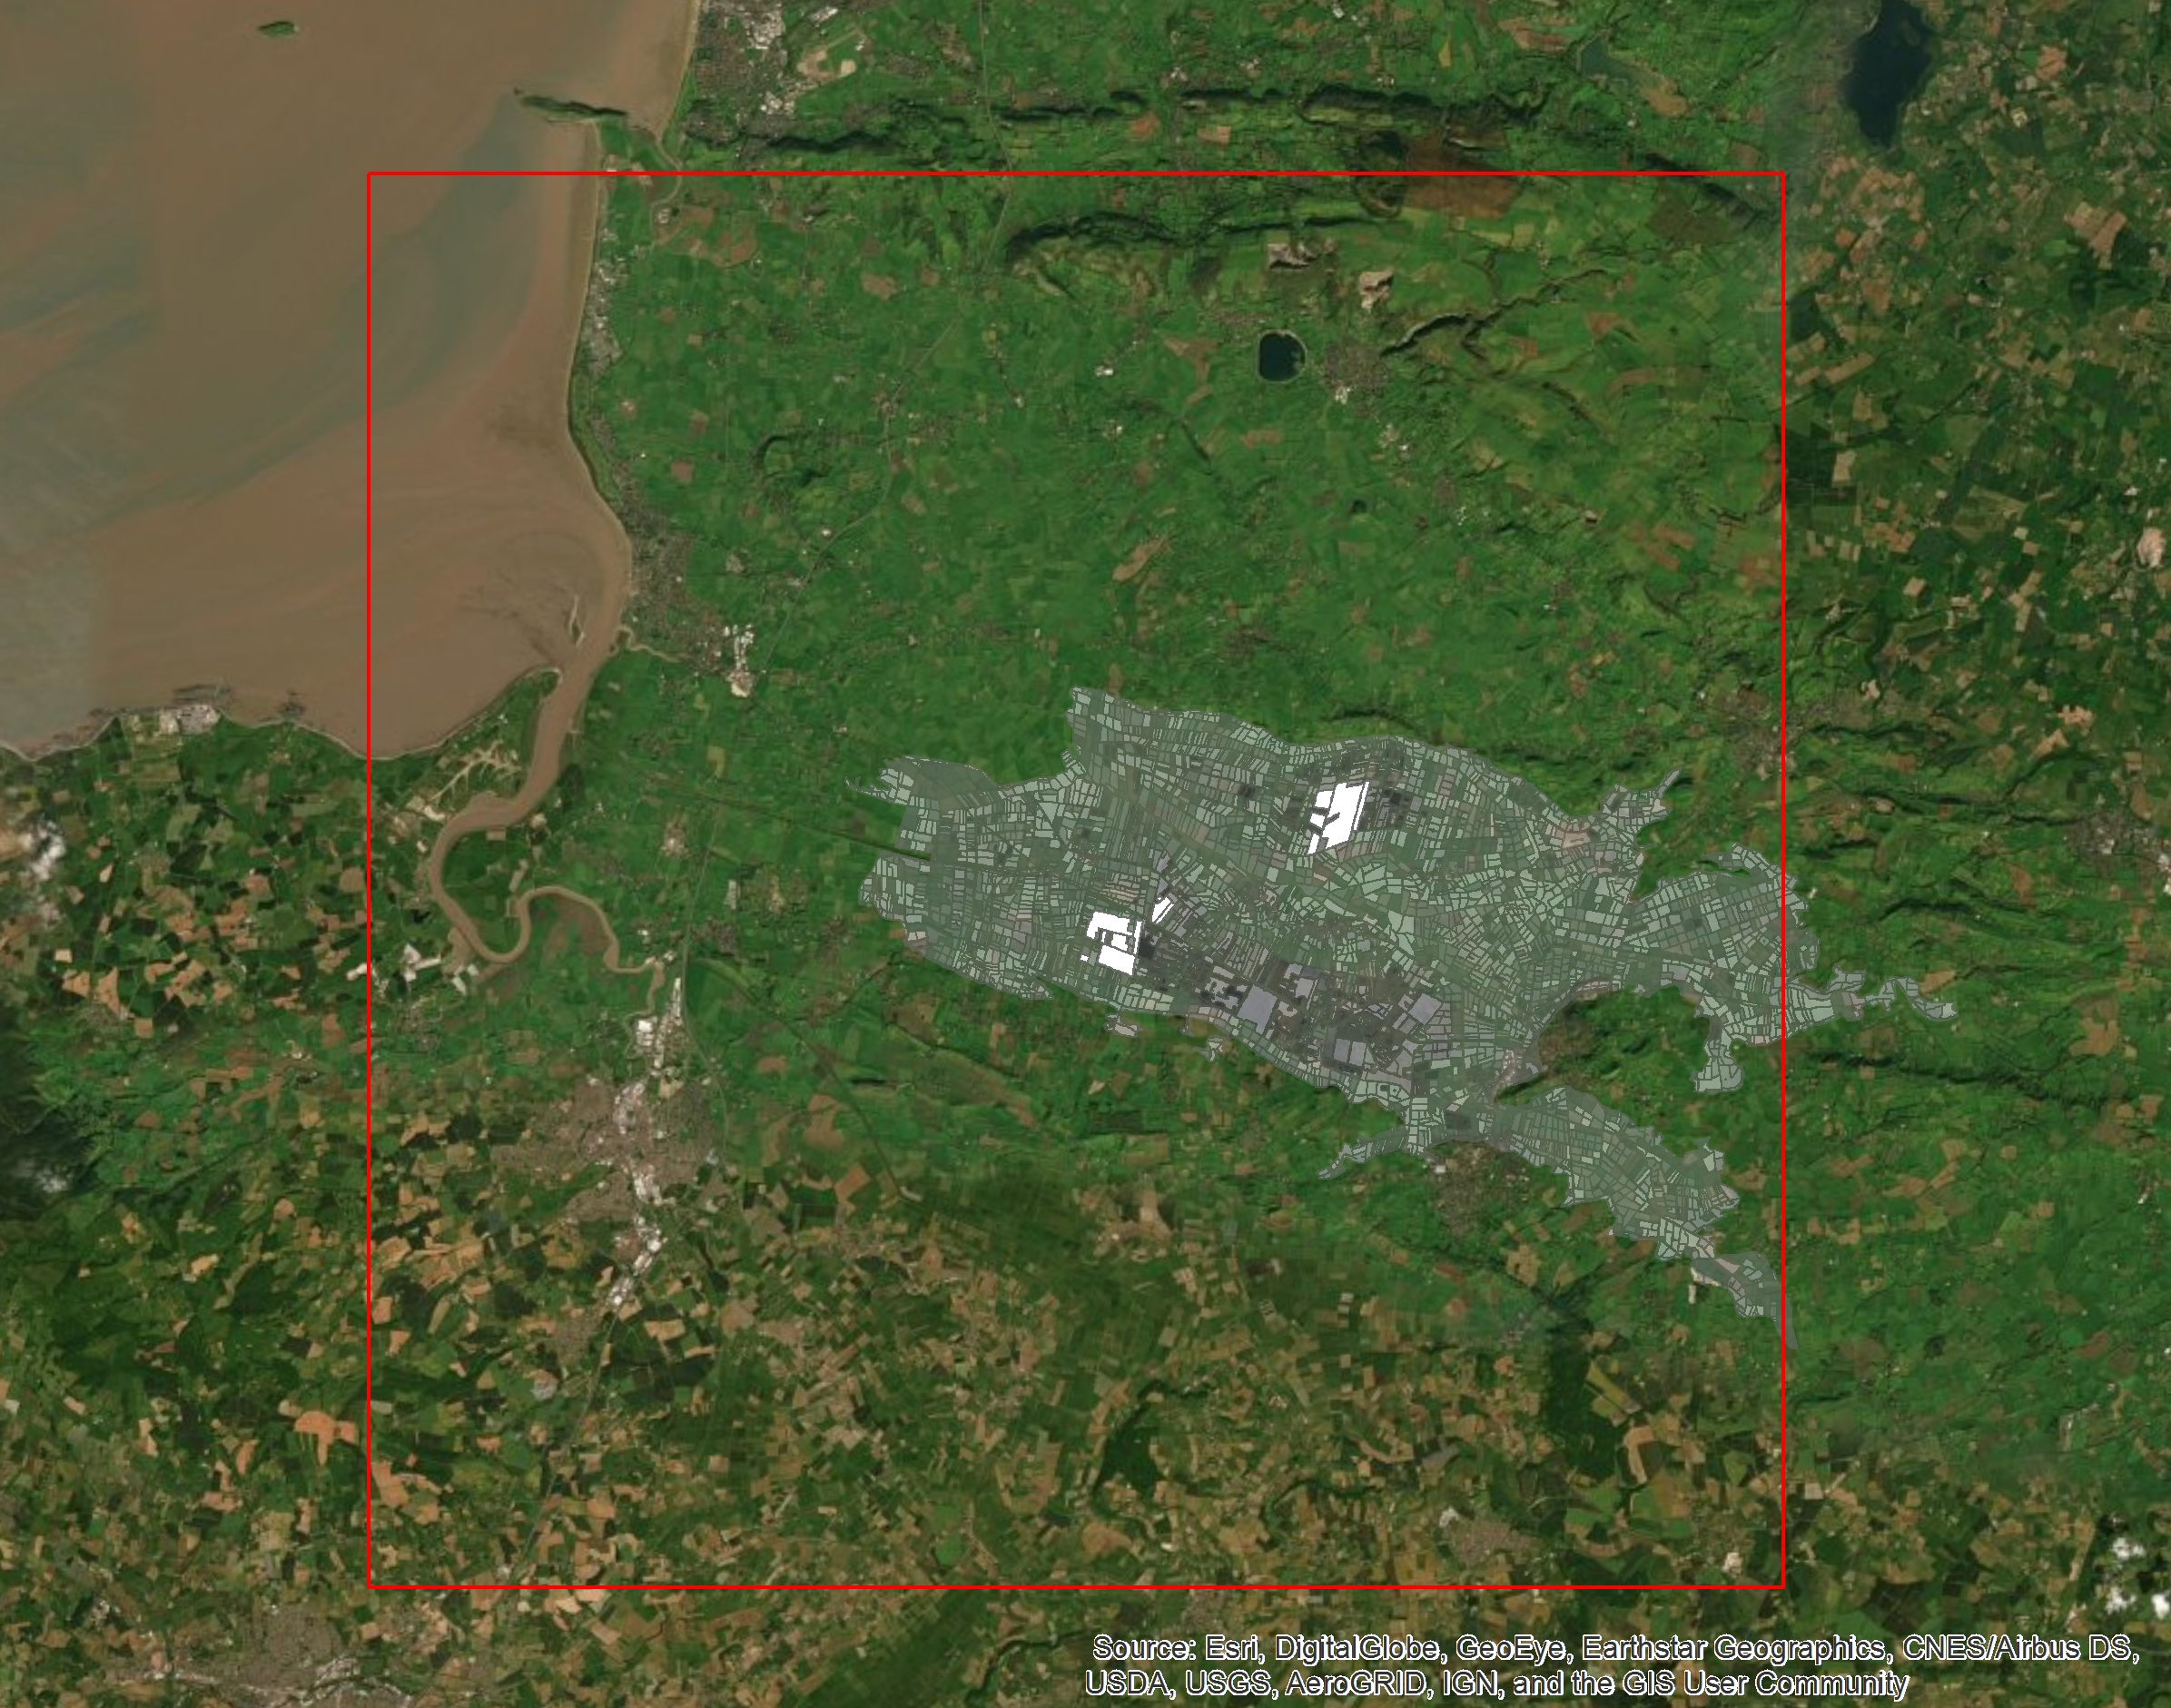
\includegraphics{WetHabitats_BoundingBoxLQ.jpg}
\caption{The bounding box for barrier analysis surrounding the Brue
Valley Living Landscape with the Somerset Wildlife Trust Avalon Marshes
reserves highlighted in white. Extents of bounding box - Top:
157637.238462m Left: 324758.957958m, Right: 354758.957958m, Bottom:
127637.238462m) Credit: Source: Esri}
\end{figure}

\hypertarget{data-preparation}{%
\subsection{Data preparation}\label{data-preparation}}

The `Open Rivers' layer on the Somerset Wildlife Trust S drive was used
to form the majority of the underlying river network. The line layer
shows most of the EA `main rivers' and streams throughout Somerset
including the River Brue, Huntspill, North Drain and South Drain. - see
S:\GIS\Layer Library\Environmental or contact the Somerset Environmental
Records Centre This was merged with the IDB viewed rhynes line layer
using the `Merge' tool to include detail of smaller arterial waterways,
ditchers and `rhynes' (local term for dicthes). The
\href{http://www.rivex.co.uk/Online-Manual/Qualitycontrolyourrivernetwork.html}{RivEX
quality control tool} was used to identify topology issues with the
river network. The following network aspects were checked; - Polyline
attributes - Zero (null) length polylines - Multi-part polylines -
Self-intersecting polylines - Disconnected polylines - Intersecting
polylines - Find cycles The resulting error log file `intersections.txt'
was used to identify and rectify false intersections within the river
network. The `Topology' tool within ArcMap was used to highlight and fix
gaps within the river network. - see
toolboxes\system toolboxes\data management tools.tbx\topology\add rule
to topology

\textless{}\textless{}\textless{}\textless{}\textless{}\textless{}\textless{}
HEAD 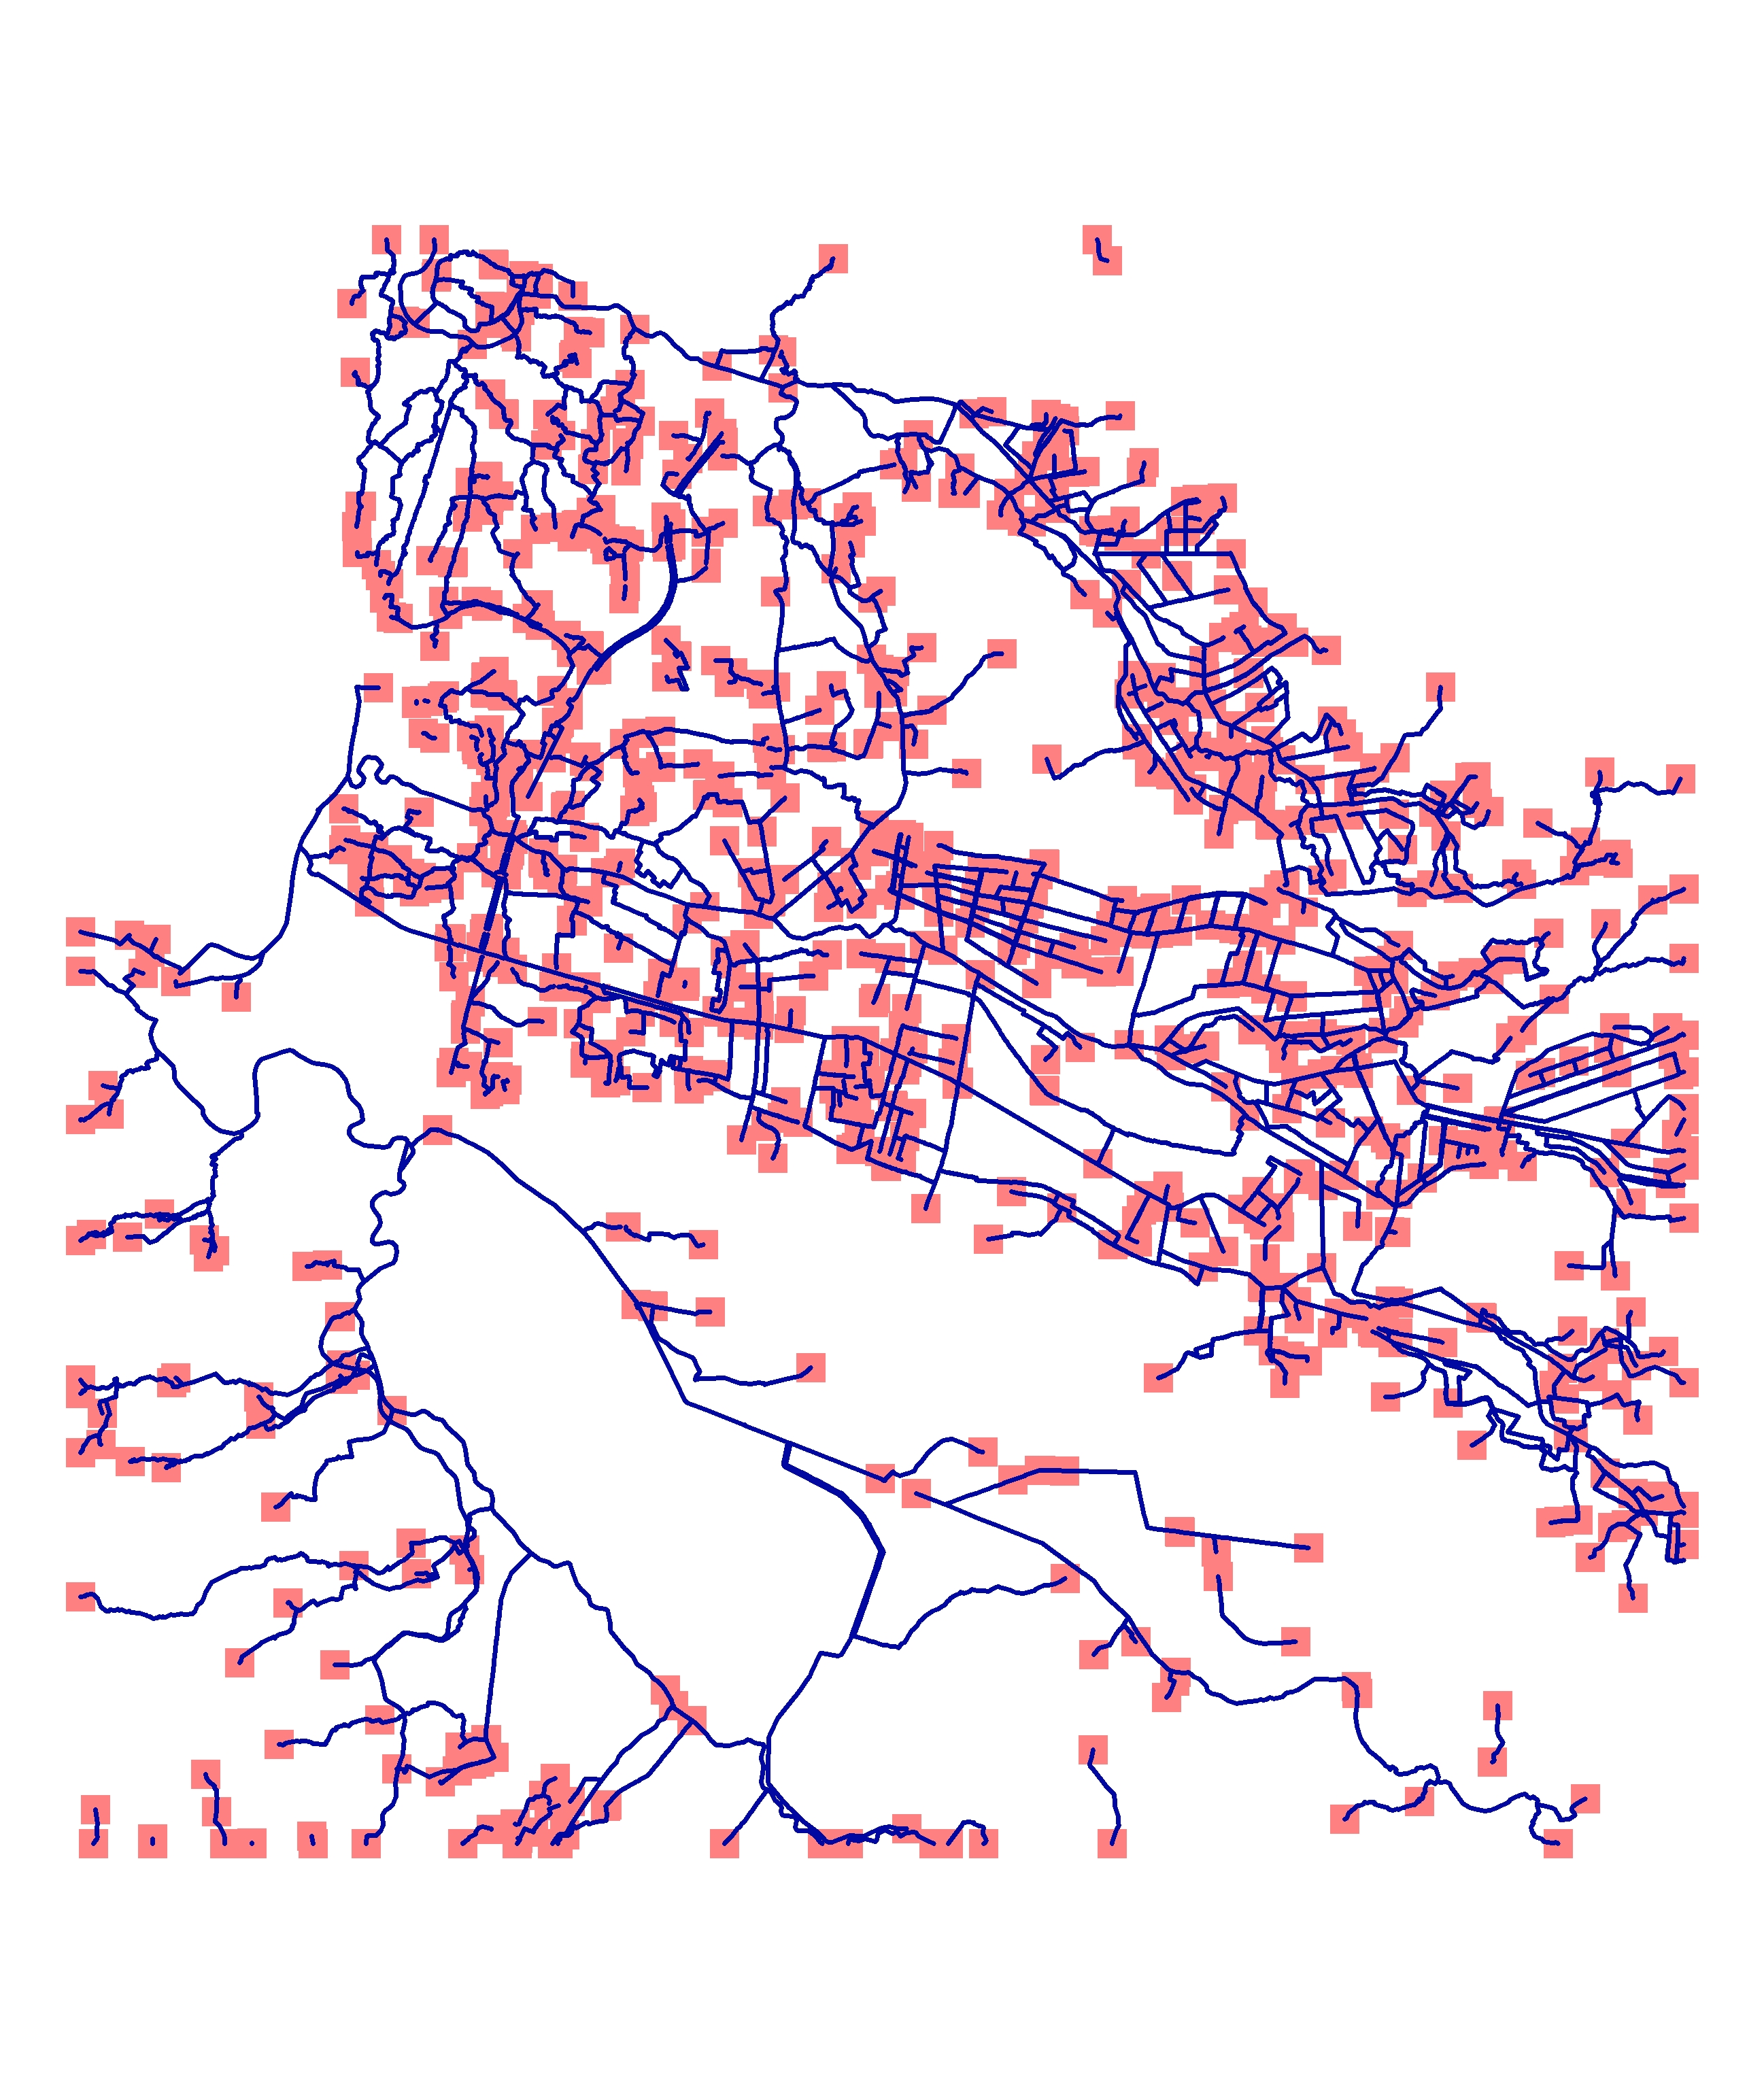
\includegraphics{AxeBrue_Topology_errors.jpg}

A screenshot showing the workflow for resolving a layer error
highlighted by the `Must not have dangles' rule is shown below.

\hypertarget{alt-text}{%
\section{\texorpdfstring{\protect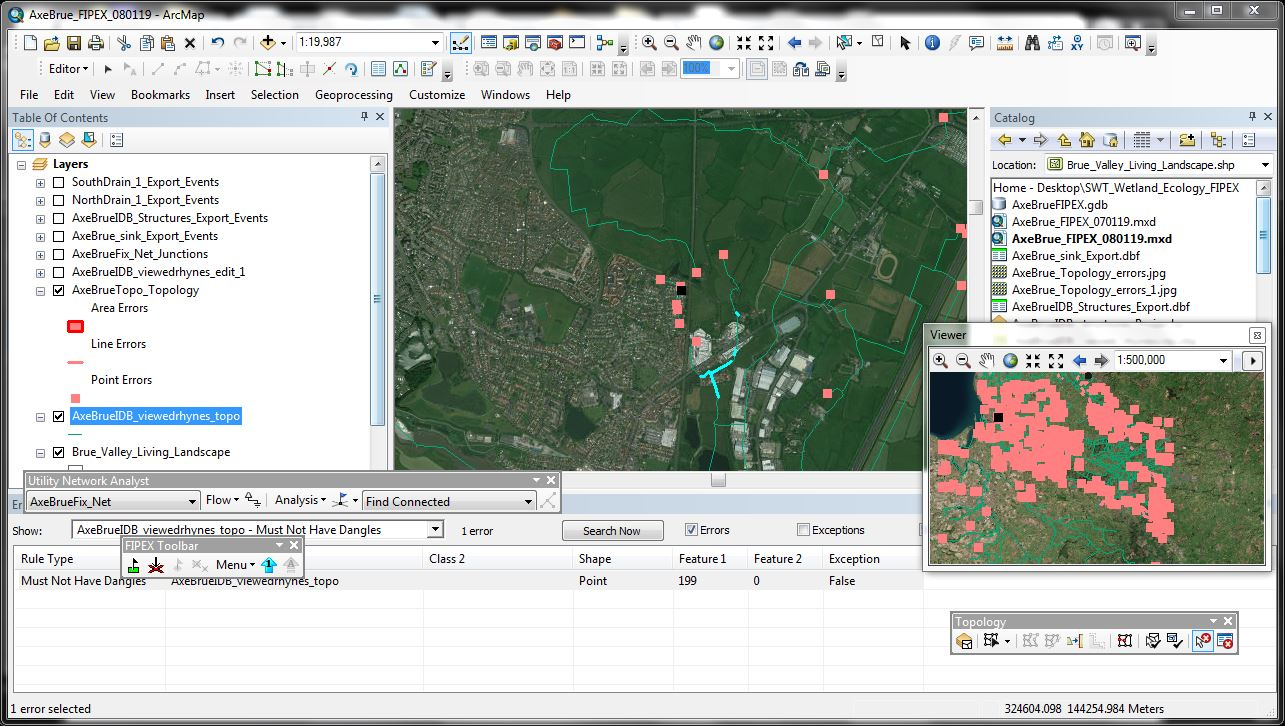
\includegraphics{AxeBrue_Topology_errors_East_of_Bridgewater_Bay.jpg}}{Alt text}}\label{alt-text}}

Brief description of `how the Somerset Moors work'.
\textgreater{}\textgreater{}\textgreater{}\textgreater{}\textgreater{}\textgreater{}\textgreater{}
285b466eaaa74fa1a331da031f9b3b8ecc8d101f

In ArcGIS, nodes represent the beginning and end of an edge. The nodes
are an important component of a network representing a river system
because they denote the locations where rivers, streams and ditches
connect to each other. The `From node' and `To node' were only present
for the IDB viewed rhynes data (`STARTNODE' and `ENDNODE'). New nodes
were created using RivEX following the `Building nodes for the first
time'
\href{http://www.rivex.co.uk/Online-Manual/Buildingnodesforthefirsttime.html}{protocol}.
The following
\href{http://www.rivex.co.uk/Online-Manual/Attributerivernetwork.html}{attributes}
were added to the river network; - Strahler order - Distance to mouth -
Upstream Accumulated Length - Catchment ID In order to represent the
movement of European Eels leaving the Brue Valley river system towards
the coast, the
\href{http://www.rivex.co.uk/Online-Manual/Reorientateanetworktoflowtomouth.html}{Re-orientate
a network to flow to mouth protocol} was followed using RivEX. By adding
arrows to the polylines users can visualise a theoretical `flow' of
mature eels migrating to the sea (layer =
AxeBrueIDB\_viewedrhynes\_singlepart\_topo). A duplicate layer was
produced showing a flipped direction of migration into the Brue System
using the `Flip line' function in ArcToolbox (layer =
AxeBrueIDB\_viewedrhynes\_singlepart\_flipped). -
toolboxes\system toolboxes\editing tools.tbx\flip line

\begin{figure}
\centering
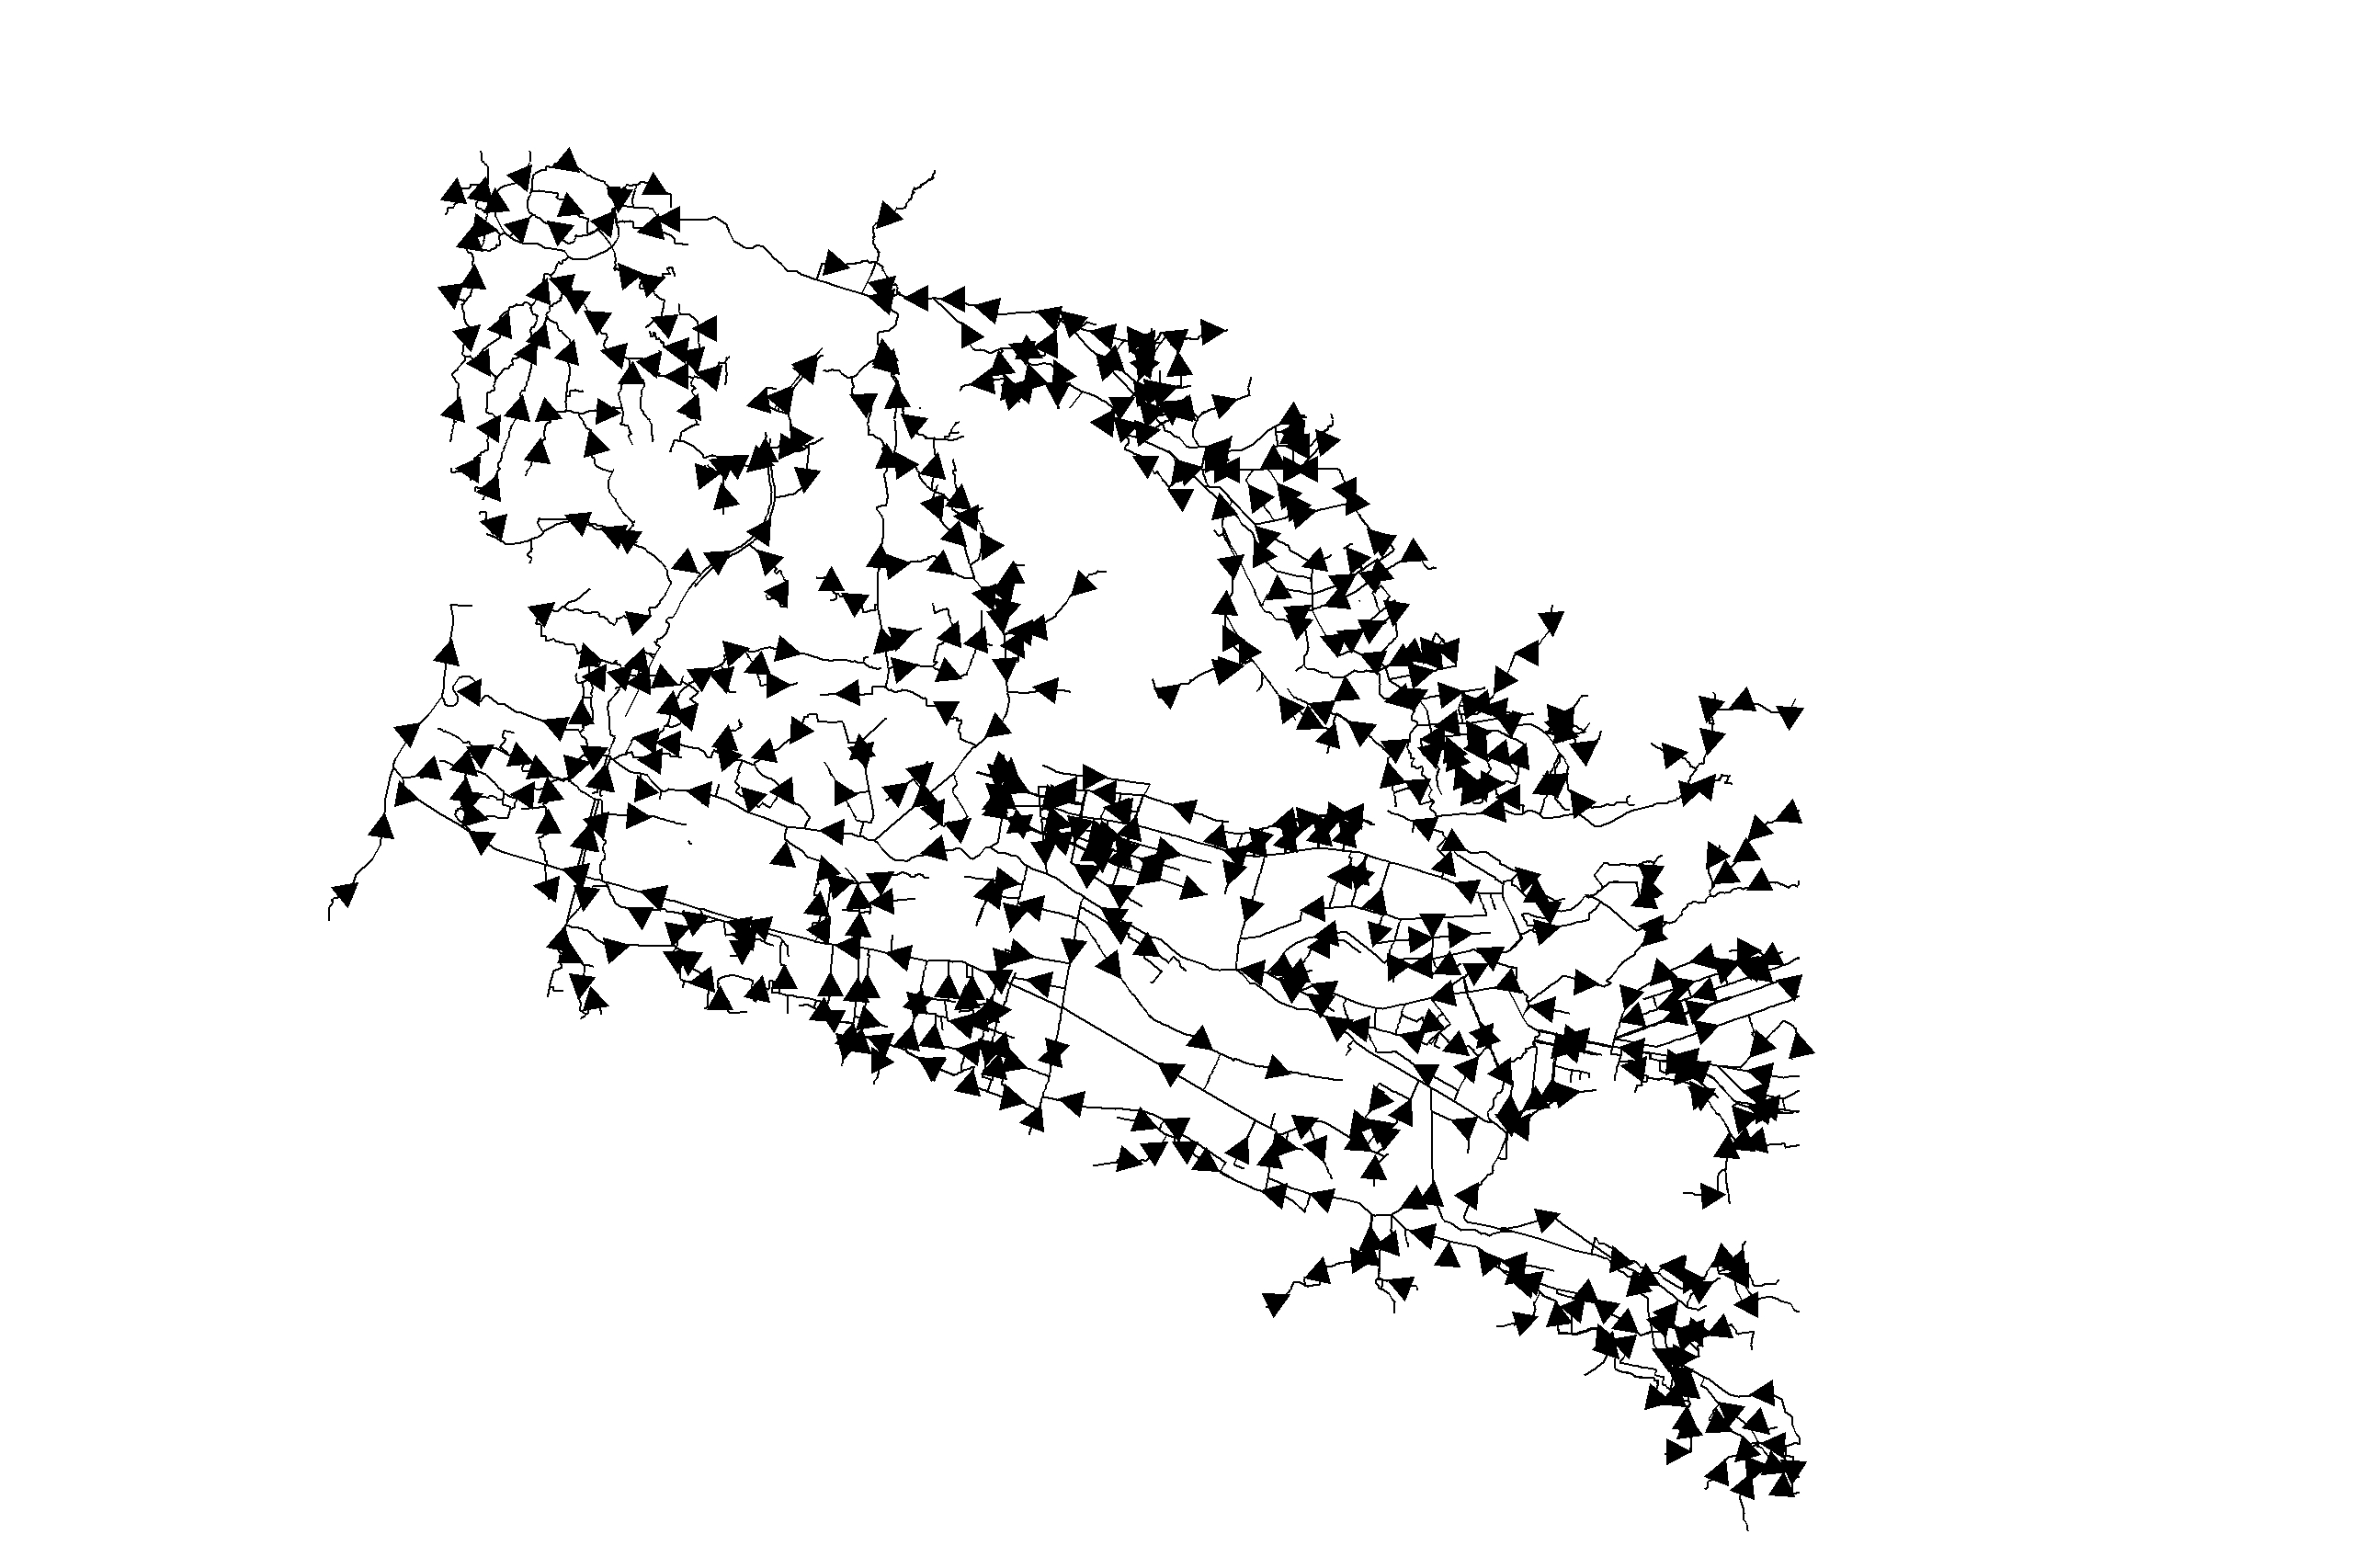
\includegraphics{AxeBrueIDB_viewedrhynes_topo.jpg}
\caption{The resulting line layer `AxeBrueIDB\_viewedrhynes\_topo'
represnting European Eel miragtion towards the sea}
\end{figure}

\textless{}\textless{}\textless{}\textless{}\textless{}\textless{}\textless{}
HEAD

\begin{verbatim}
## Warning: package 'knitr' was built under R version 3.6.1
\end{verbatim}

\begin{verbatim}
## Warning: package 'kableExtra' was built under R version 3.6.1
\end{verbatim}

\textbackslash{}begin\{table\}{[}t{]}

\textbackslash{}caption\{\label{tab:unnamed-chunk-2}The first five rows
of `AxeBrueIDB\_viewedrhynes\_singlepart\_topo.csv' attribute table for
polyline layer of river system representing migration towards the
coast\} \centering

\begin{tabular}{l|r|l|l|r|r|l|r|r|l|l|l|l|r|l|r|r|r|r|r|r|r|r|r|r|r|r|r|l|r|r|r|r|l|r|r|r|r|r|r|r|r|r|r|r|r|r|r|r}
\hline
  & OBJECTID\_12 & Name & C\_O & id2 & length\_m & IDENTIFIER & STARTNODE & ENDNODE & FORM & NUMBER & FLOWDIRCTN & FICTITIOUS & LENGTH & ALTNAME & Shape\_Leng & Shape\_Le\_1 & Enabled & Shape\_Le\_2 & OBJECTID & CatchID & Strahler & Segment & Dist2Mth & Reach & ORIG\_FID & Fnode & Tnode & Flipped & Fnode1 & Tnode1 & Fnode2 & Tnode2 & Flipped2 & Fnode3 & Tnode3 & US\_Accum & Dist2Mth2 & US\_Accum2 & CatchID2 & Fnode4 & Tnode4 & Dist2Mth3 & CatchID3 & US\_Accum3 & Dist2Mth4 & CatchID4 & US\_Accum4 & Shape\_Length\\
\hline
1 & 1 & Abbeyshard Rhyne &  & 1 & 655 &  & 0 & 0 &  & NA &  &  & 0 & NA & 0 & 655.3142 & 1 & 655.3142 & 1 & 443 & 1 & 669 & 1190.6407 & 11221 & 1 & 1 & 2 & Not visited & 1 & 2 & 1 & 2 & Not visited & 1 & 2 & 1190.6407 & 1190.6407 & 1190.6407 & 511 & 1 & 2 & 1190.6407 & 623 & 1190.6407 & 1190.6407 & 623 & 1190.6407 & 1190.6408\\
\hline
2 & 2 & Actis Rhyne &  & 2 & 1895 &  & 0 & 0 &  & NA &  &  & 0 & NA & 0 & 1894.8583 & 1 & 1952.9903 & 2 & 442 & 1 & 668 & 1965.7188 & 11221 & 2 & 3 & 4 & Not visited & 3 & 4 & 3 & 4 & Not visited & 3 & 4 & 1965.7188 & 1965.7188 & 1965.7188 & 510 & 3 & 4 & 1965.7188 & 622 & 1965.7188 & 1965.7188 & 622 & 1965.7188 & 1965.7188\\
\hline
3 & 3 & Aldershard Rhyne &  & 3 & 1246 &  & 0 & 0 &  & NA &  &  & 0 & NA & 0 & 1245.6051 & 1 & 1280.6141 & 3 & 280 & 1 & 428 & 1420.4883 & 11221 & 3 & 5 & 6 & Not visited & 5 & 6 & 5 & 6 & Not visited & 5 & 6 & 1259.0172 & 1420.4883 & 1259.0172 & 306 & 5 & 6 & 1259.0172 & 621 & 1420.4883 & 1259.0172 & 621 & 1420.4883 & 1259.0172\\
\hline
4 & 4 & Aller Moor Drove Rhyne 08 &  & 4 & 832 &  & 0 & 0 &  & NA &  &  & 0 & NA & 0 & 832.4268 & 1 & 832.4268 & 4 & 441 & 1 & 116 & 834.3546 & 11221 & 4 & 7 & 8 & Not visited & 7 & 8 & 7 & 8 & Not visited & 7 & 8 & 421.5742 & 421.5742 & 421.5742 & 509 & 7 & 8 & 421.5742 & 620 & 421.5742 & 421.5742 & 620 & 421.5742 & 421.5742\\
\hline
5 & 5 & Aller Moor Drove Rhyne 08 &  & 4 & 832 &  & 0 & 0 &  & NA &  &  & 0 & NA & 0 & 832.4268 & 1 & 832.4268 & 5 & 441 & 1 & 116 & 834.3546 & 11221 & 4 & 9 & 10 & Not visited & 9 & 10 & 9 & 10 & Not visited & 9 & 10 & 412.7804 & 412.7804 & 412.7804 & 508 & 9 & 10 & 412.7804 & 619 & 412.7804 & 412.7804 & 619 & 412.7804 & 412.7804\\
\hline
\end{tabular}

\textbackslash{}end\{table\} Known water control structures as managed
by the Environment Agency and Somerset Internal Drainage Board were
plotted as a point layer in ArcMap. The base layer used during
geographic information system analysis is a merge of
\href{https://www.arcgis.com/apps/View/index.html?appid=22497f115856472eb9e58fdba3023191}{`AxeBrueIDB\_structures'}
and structures from the Somerset Internal Drainage Board water level
\href{http://somersetdrainageboards.gov.uk/environment/wlmps/}{management
plans} (WLMPs) for the North Drain and South Drain. Structure management
information showing when structures were open or closed was only
available for 24\% of the final dataset (N = 103).

Water Control structure data and sources

Filename

Contributor

Link

Structures

1

AxeBrueIDB

Somerset Internal Drainage Board

\url{https://www.arcgis.com/apps/View/index.html?appid=22497f115856472eb9e58fdba3023191}

IDB watercourse and structure GI data.ÿ

2

South Drain Perm

IDB South Drain Water Level Management Plan

\url{http://www.somersetdrainageboards.gov.uk/media/South-Drain-WLMP-Brue-Approved-Apr-10.pdf}

IDB and Environment Agency strutcure data

3

North Drain WLMP Winter and Summer Levels

IDB North Drain Water Level Management Plan

\url{https://somersetdrainageboards.gov.uk/media/North-Drain-WLMP-Brue-Approved-Apr-10.pdf}

IDB and Environment Agency strutcure data

The locations of water control structures from all three sources were
viewed as point layers in ESRI ArcMap (v. 10.6) before being merged
using the `Merge' tool in ArcToolbox. The field map was left unchanged.
- toolboxes\system toolboxes\data management tools.tbx\general\merge

\begin{figure}
\centering
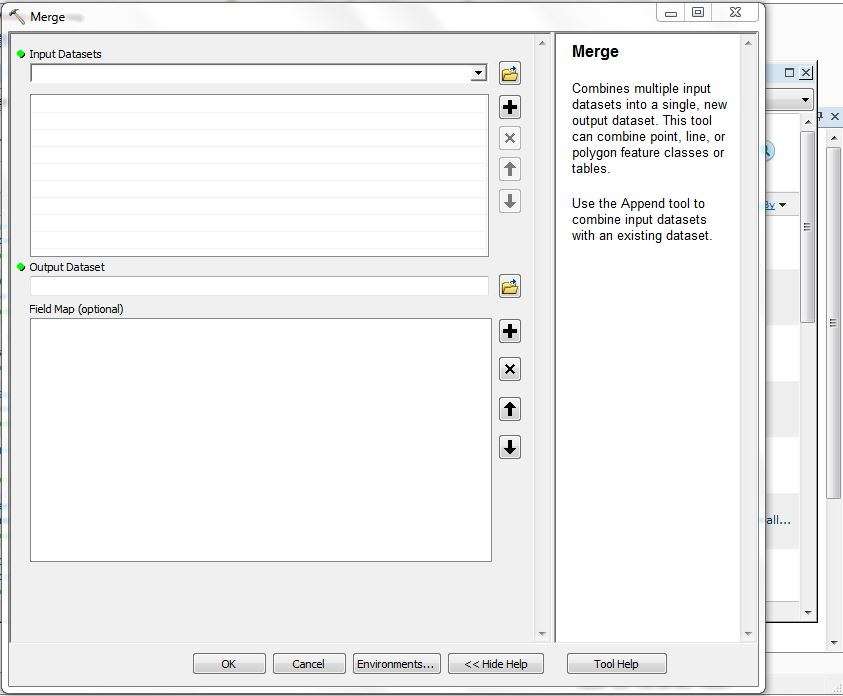
\includegraphics{Capture_MergeTool.jpg}
\caption{Alt text}
\end{figure}

\textbackslash{}begin\{table\}{[}t{]}

\textbackslash{}caption\{\label{tab:unnamed-chunk-4}The first five rows
of `AxeBrue\_IDB\_merged\_140219\_Snapped.csv' table which shows all
structures included in the analysis\} \centering

\begin{tabular}{l|r|r|r|l|l|l|l|l|l|r|r|r|r|l|r|r|r|r|r|l|r|l|l|r|r|r|r|l|l|l}
\hline
  & OBJECTID\_12 & OBJECTID & ObjectID\_1 & Water\_leve & Grid\_ref\_ & Owned\_by & Operated\_b & Watercours & Descriptio & X & Y & Lat & Long\_ & Source & Enabled & NEAR\_FID & NEAR\_DIST & NEAR\_X & NEAR\_Y & Dimensions & FID\_1 & Structure & structure\_ & Count\_ & AncillaryR & AncillaryRole & SnapDist & ForcedMove & SnapQual & SrchName\\
\hline
1 & 1 & 1 & 1 &  & NA & EA & EA & River Brue & Pair of lifting sluices with tilting crests & 333230 & 146210 & 0 & 51.21117 & South Drain & 1 & 59 & 31.96019 & 334332.5 & 147840.3 &  & NA &  & Unknown & NA & NA & NA & 0.00 & N & Nearest Polyline, no name check & n/a\\
\hline
2 & 2 & 2 & 2 & Highbridge Clyse & NA & Private & Private & River Brue & Two vertical lifting gates and two tidal & 331350 & 147240 & 0 & 51.22021 & South Drain & 1 & 371 & 157.64445 & 330720.7 & 146633.7 &  & NA &  & Unknown & NA & NA & NA & 0.00 & N & Nearest Polyline, no name check & n/a\\
\hline
3 & 3 & 3 & 3 & Gold Corner Pumping Station & NA & EA & EA & South Drain & Pumping Station & 336720 & 143040 & 0 & 51.18307 & South Drain & 1 & 186 & 36.48692 & 337437.8 & 143744.8 &  & NA &  & Pumping Station & NA & NA & NA & 0.02 & N & Nearest Polyline, no name check & n/a\\
\hline
4 & 4 & 4 & 4 & Shaking Drove Tilting Weir & NA & EA & EA & South Drain & Tilting weir and a flap & 336800 & 143170 & 0 & 51.18425 & South Drain & 1 & 186 & 36.48692 & 337437.8 & 143744.8 &  & NA &  & Tilting Weir & NA & NA & NA & 0.02 & N & Nearest Polyline, no name check & n/a\\
\hline
5 & 5 & 5 & 5 & Huntspill Sluice & NA & EA & EA & Huntspill River & Two pairs of vertical
lifting gates & 329260 & 145730 & 0 & 51.20638 & South Drain & 1 & 371 & 157.64445 & 330720.7 & 146633.7 &  & NA &  & Unknown & NA & NA & NA & 0.00 & N & Nearest Polyline, no name check & n/a\\
\hline
\end{tabular}

\textbackslash{}end\{table\}

The RivEX
\href{http://www.rivex.co.uk/Online-Manual/Snapsitestonetwork.html}{snapping
sites to network tool} was used to ensure that the point layer
overlapped the polyline layer. A snapping tolerance of 20m was used.

\#RivEX analysis

Barrier analysis was carried out using a river network tool RivEX (v
10.28) with ESRI ArcMap (v. 10.6). RivEX is an ESRI ArcGIS 10.6 tool for
processing vector river networks. It has tools for quality control,
stream ordering, sampling and site linking. Following the
\href{http://www.rivex.co.uk/Online-Manual/Distancesbetweendamsaworkedexamp.html}{`Distances
between dams worked example'} the amount of habitat available for each
water control structure was calculated and added as a seperate column to
the point layer's attribute table. This was then visualised in ArcMap by
changing the layer symbology using a colour gradient with 10 natural
breaks to allow users to prioritise structures by showing the amount of
potential habitat that would be opened up if a fish pass was added.

\textbackslash{}begin\{table\}{[}t{]}

\textbackslash{}caption\{\label{tab:unnamed-chunk-5}The first five rows
of `AxeBrue\_IDB\_DS\_160219' attribute table showing the additional
column for `AvailDSnet showing the amount of available habitat in a
'downstream' or Westerly direction\} \centering

\begin{tabular}{l|r|r|l|l|l|l|l|l|r|r|r|r|l|r|r|r|r|r|l|r|l|l|r|r|r|r|l|l|l|r|r|r|r|r|r|r|r|r}
\hline
  & OBJECTID & AxeBrue\_IDB\_merged\_140219\_Snapped\_OBJECTID & AxeBrue\_IDB\_merged\_140219\_Snapped\_Water\_leve & AxeBrue\_IDB\_merged\_140219\_Snapped\_Grid\_ref\_ & AxeBrue\_IDB\_merged\_140219\_Snapped\_Owned\_by & AxeBrue\_IDB\_merged\_140219\_Snapped\_Operated\_b & AxeBrue\_IDB\_merged\_140219\_Snapped\_Watercours & AxeBrue\_IDB\_merged\_140219\_Snapped\_Descriptio & AxeBrue\_IDB\_merged\_140219\_Snapped\_X & AxeBrue\_IDB\_merged\_140219\_Snapped\_Y & AxeBrue\_IDB\_merged\_140219\_Snapped\_Lat & AxeBrue\_IDB\_merged\_140219\_Snapped\_Long\_ & AxeBrue\_IDB\_merged\_140219\_Snapped\_Source & AxeBrue\_IDB\_merged\_140219\_Snapped\_Enabled & AxeBrue\_IDB\_merged\_140219\_Snapped\_NEAR\_FID & AxeBrue\_IDB\_merged\_140219\_Snapped\_NEAR\_DIST & AxeBrue\_IDB\_merged\_140219\_Snapped\_NEAR\_X & AxeBrue\_IDB\_merged\_140219\_Snapped\_NEAR\_Y & AxeBrue\_IDB\_merged\_140219\_Snapped\_Dimensions & AxeBrue\_IDB\_merged\_140219\_Snapped\_FID\_1 & AxeBrue\_IDB\_merged\_140219\_Snapped\_Structure & AxeBrue\_IDB\_merged\_140219\_Snapped\_structure\_ & AxeBrue\_IDB\_merged\_140219\_Snapped\_Count\_ & AxeBrue\_IDB\_merged\_140219\_Snapped\_AncillaryR & AxeBrue\_IDB\_merged\_140219\_Snapped\_AncillaryRole & AxeBrue\_IDB\_merged\_140219\_Snapped\_SnapDist & AxeBrue\_IDB\_merged\_140219\_Snapped\_ForcedMove & AxeBrue\_IDB\_merged\_140219\_Snapped\_SnapQual & AxeBrue\_IDB\_merged\_140219\_Snapped\_SrchName & AxeBrue\_IDB\_merged\_140219\_Snapped\_Reach & AxeBrueIDB\_Sum\_Output\_OBJECTID & AxeBrueIDB\_Sum\_Output\_FREQUENCY & AxeBrueIDB\_Sum\_Output\_SiteID & DistFromLn & DistAlngLn & USLength & SUM\_USLength & AvailDSNet\\
\hline
1 & 1 & 1 &  & NA & EA & EA & River Brue & Pair of lifting sluices
with tilting crests & 333230 & 146210 & 0 & 51.21117 & South Drain & 1 & 59 & 31.96019 & 334332.5 & 147840.3 &  & NA &  &  & NA & NA & NA & 0.00 & N & Nearest Polyline, no name check & n/a & 11221 & 1 & 1 & 1 & 1.06e-05 & 0.0754126 & 219.7921 & 0 & 219.7921\\
\hline
2 & 2 & 2 & Highbridge Clyse & NA & Private & Private & River Brue & Two vertical lifting gates and two tidal & 331350 & 147240 & 0 & 51.22021 & South Drain & 1 & 371 & 157.64445 & 330720.7 & 146633.7 &  & NA &  &  & NA & NA & NA & 0.00 & N & Nearest Polyline, no name check & n/a & 11221 & 2 & 1 & 2 & 0.00e+00 & 0.5781129 & 1437.6084 & 0 & 1437.6084\\
\hline
3 & 3 & 3 & Gold Corner Pumping Station & NA & EA & EA & South Drain & Pumping Station & 336720 & 143040 & 0 & 51.18307 & South Drain & 1 & 186 & 36.48692 & 337437.8 & 143744.8 &  & NA &  &  & NA & NA & NA & 0.02 & N & Nearest Polyline, no name check & n/a & 11221 & 3 & 1 & 3 & 1.14e-05 & 0.1748863 & 618.9204 & 0 & 618.9204\\
\hline
4 & 4 & 4 & Shaking Drove Tilting Weir & NA & EA & EA & South Drain & Tilting weir and a flap & 336800 & 143170 & 0 & 51.18425 & South Drain & 1 & 186 & 36.48692 & 337437.8 & 143744.8 &  & NA &  &  & NA & NA & NA & 0.02 & N & Nearest Polyline, no name check & n/a & 11221 & 4 & 1 & 4 & 1.14e-05 & 0.1748863 & 618.9204 & 0 & 618.9204\\
\hline
5 & 5 & 5 & Huntspill Sluice & NA & EA & EA & Huntspill River & Two pairs of vertical
lifting gates & 329260 & 145730 & 0 & 51.20638 & South Drain & 1 & 371 & 157.64445 & 330720.7 & 146633.7 &  & NA &  &  & NA & NA & NA & 0.00 & N & Nearest Polyline, no name check & n/a & 11221 & 5 & 1 & 5 & 0.00e+00 & 0.5781129 & 1437.6084 & 0 & 1437.6084\\
\hline
\end{tabular}

\textbackslash{}end\{table\} A draft version of the map was sent out to
project partners and potential users for feedback including the
Environment Agency, Sustainable Eel Group, Westcountry Rivers Trust and
Somerset Wildlife Trust. ======= The base layer is a merge of
`AxeBrueIDB\_structures' and structures from the Internal Drainage Board
management plans for the North Drain and South Drain.
\url{https://www.arcgis.com/apps/View/index.html?appid=22497f115856472eb9e58fdba3023191}
\url{http://somersetdrainageboards.gov.uk/environment/wlmps/\%5BIDB2010\%5D}
{[}Brue2010{]}
\textgreater{}\textgreater{}\textgreater{}\textgreater{}\textgreater{}\textgreater{}\textgreater{}
285b466eaaa74fa1a331da031f9b3b8ecc8d101f

\hypertarget{results}{%
\section{Results}\label{results}}

The final layers used during analysis included 433 water control
structures within the study area. Penstocks were the most frequent
structure type included in the barrier analysis (N=103). Outlets and
spillways were the least frequent structure type in the study area
(N=1). 48 structures did not any of the major structure types from their
descriptions.

\begin{verbatim}
## Warning: package 'ggplot2' was built under R version 3.6.1
\end{verbatim}

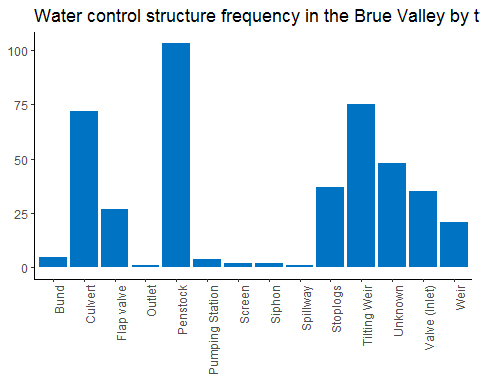
\includegraphics{EelHabitatMapMardown_files/figure-latex/unnamed-chunk-6-1.pdf}

Most structures included in the analysis can be found in the South Drain
catchment (N=25). Structure density is lowest on the River Yeo and
Shipham Rhyne.

\hypertarget{water-control-structure-density-by-catchment}{%
\section{\texorpdfstring{\protect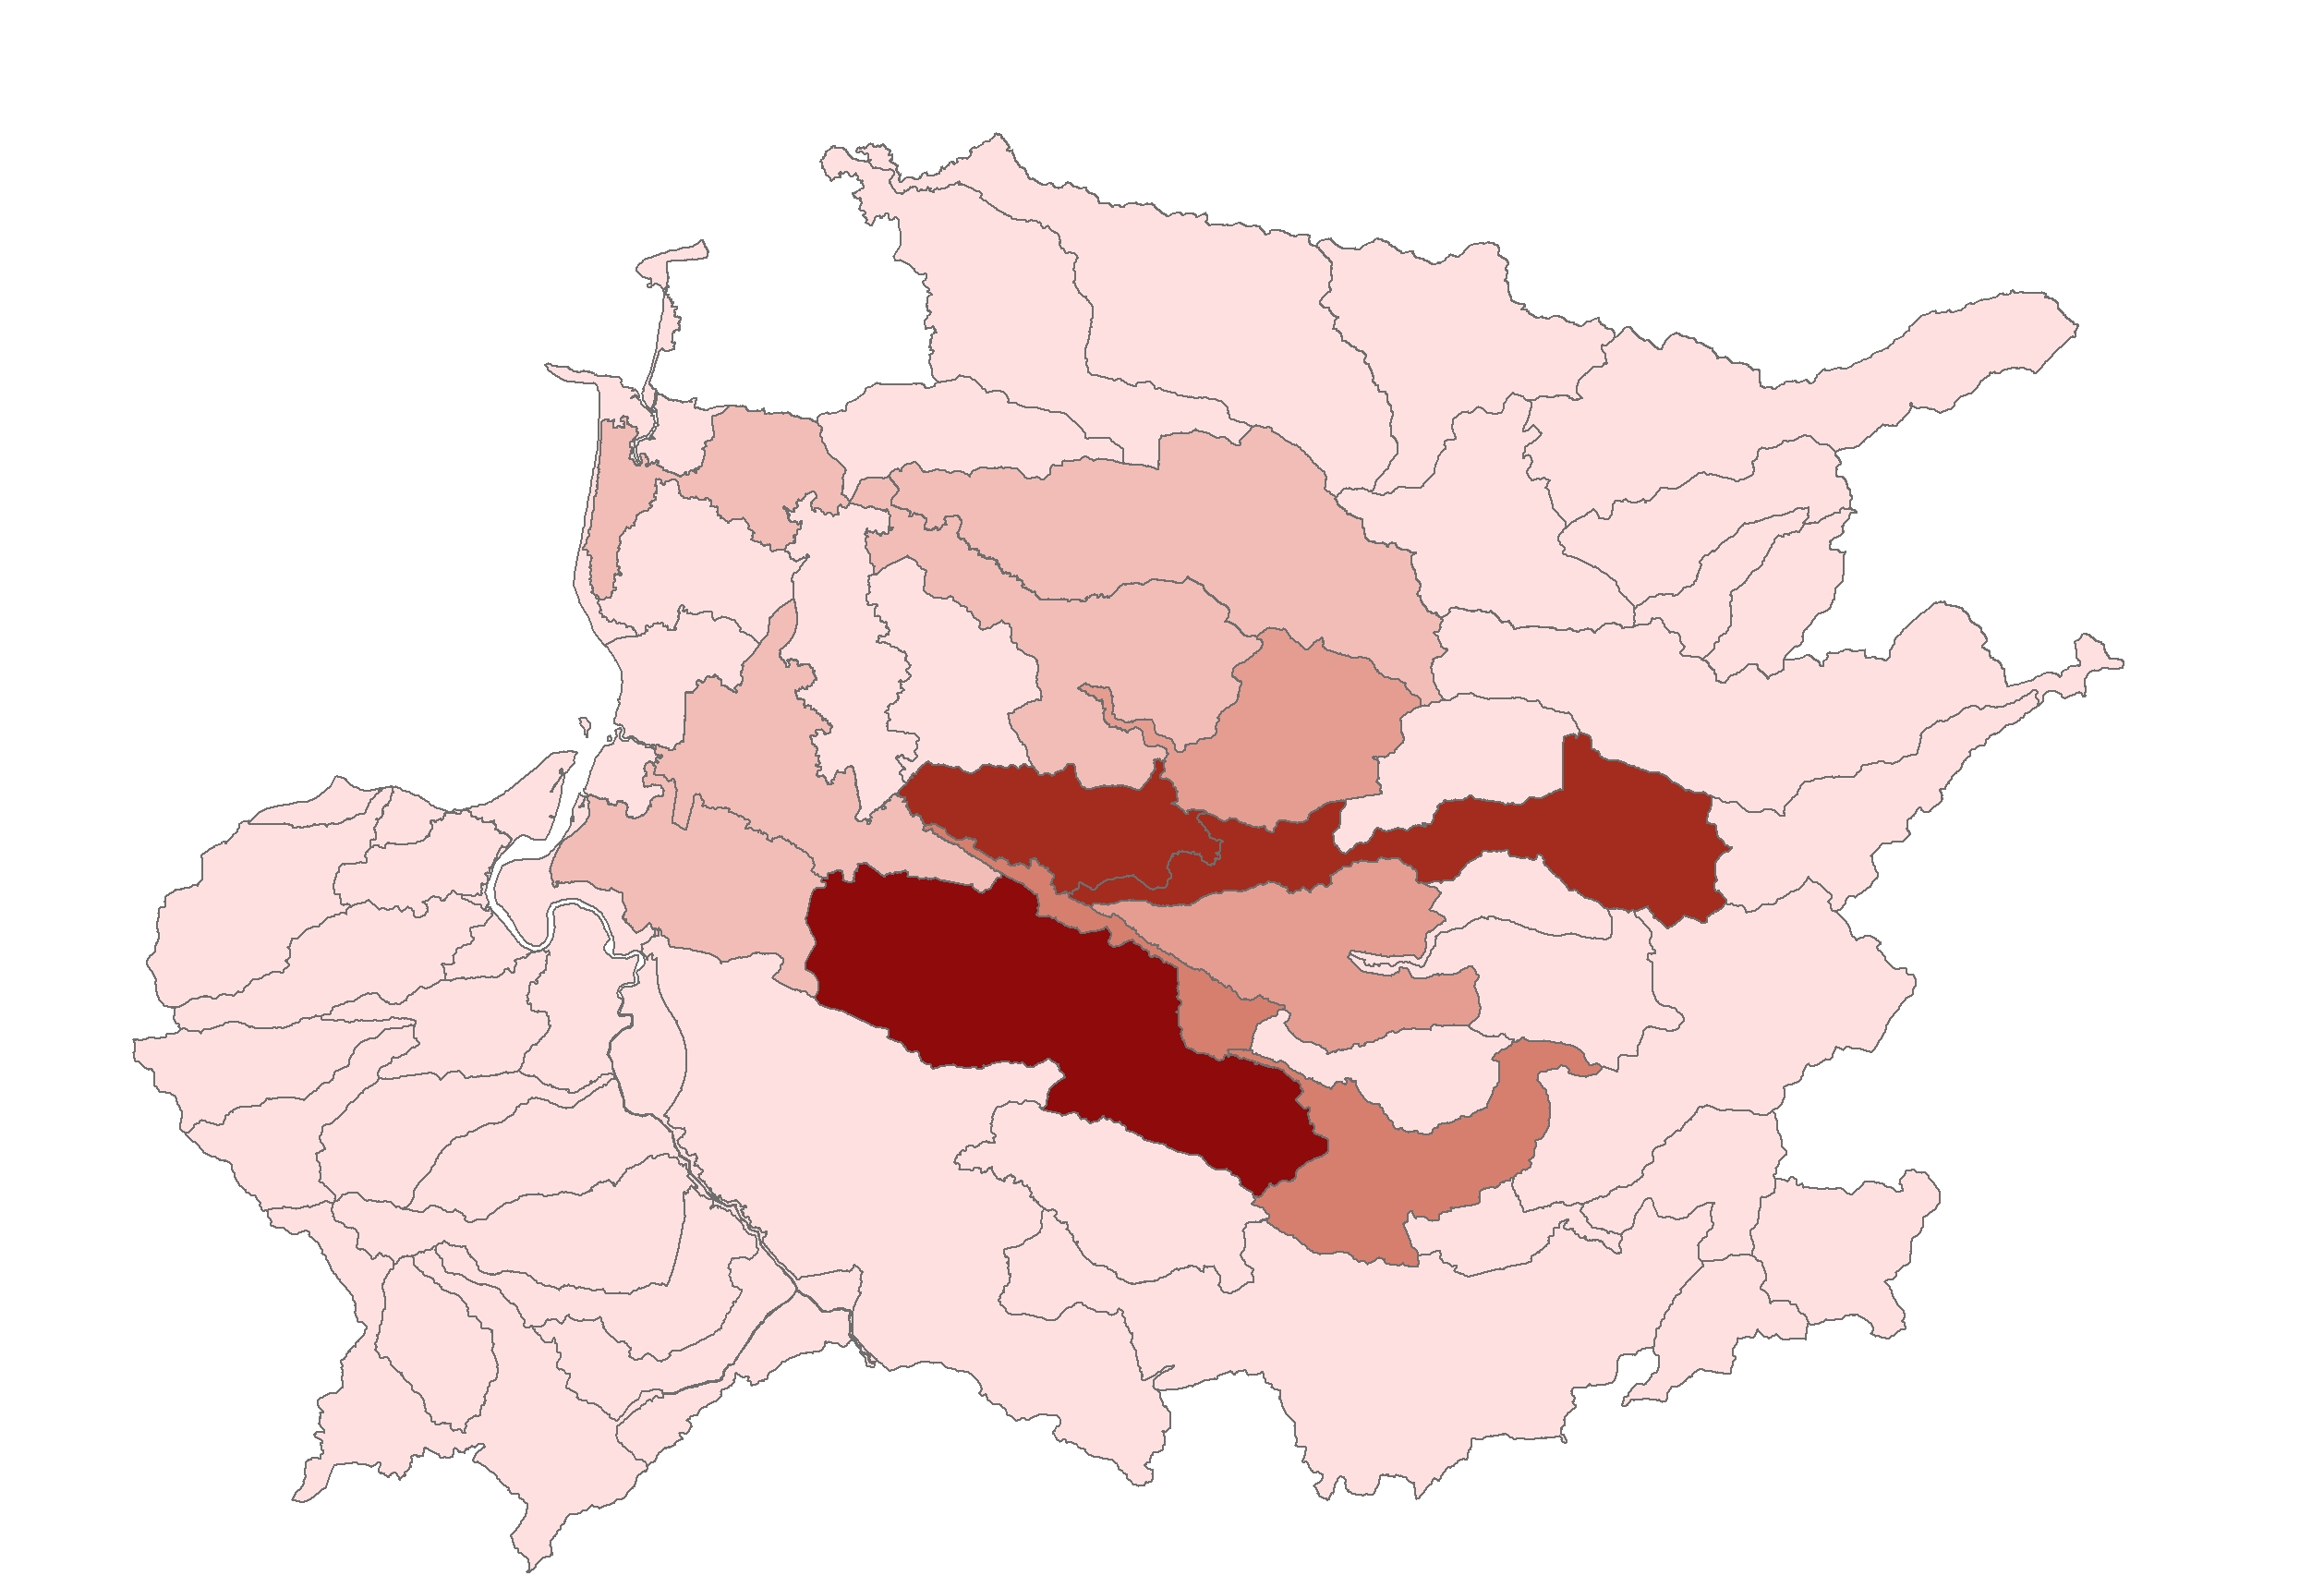
\includegraphics{AxeBrue_RIVEX_190219_StructureDen_.jpg}}{Water control structure density by catchment}}\label{water-control-structure-density-by-catchment}}

The resulting habitat maps can be viewed on
\href{http://arcg.is/8qavW}{ArcGIS online}. The final layer used during
analysis included 433 water control structures within the study area.
Stream and downstream habitat availability of water control structures
managed by the Internal Drainage Board and Environment Agency.

Darker points show structures that have the potential for releasing the
most habitat downstream or upstream if modified for fish passability.

These layers do not account for the quality of `available habitat'
upstream/downstream. Habitat availability is based on the assumption
that all underlying habitat is suitable for European Eel. In the absence
of detailed biological information or appropriate models of habitat
quality this is a common approach (see
{[}Buddendorf2017a{]}{[}Cote2009{]}{[}Grill2014{]}{[}Sheer2006{]}). At
this point the layers also fail to account for the management of
individual structures. For example, a structure closed during Winter
Penn is likely to restrict access to all habitat downstream for eels
moving through the system. SWT plans to include information on the
potential financial cost of improving structure permeability in future
iterations of the eel passability scores.
\textgreater{}\textgreater{}\textgreater{}\textgreater{}\textgreater{}\textgreater{}\textgreater{}
285b466eaaa74fa1a331da031f9b3b8ecc8d101f

\begin{table}[t]

\caption{\label{tab:unnamed-chunk-7}The top 10 structures highlighted by the habitat map with the greatest available habitat in a 'downstream' or Westerly direction}
\centering
\begin{tabular}{l|r|r|l|l|l|l|l|l|r|r|r|r|l|r|r|r|r|r|l|r|l|l|r|r|r|r|l|l|l|r|r|r|r|r|r|r|r|r}
\hline
  & OBJECTID & AxeBrue\_IDB\_merged\_140219\_Snapped\_OBJECTID & AxeBrue\_IDB\_merged\_140219\_Snapped\_Water\_leve & AxeBrue\_IDB\_merged\_140219\_Snapped\_Grid\_ref\_ & AxeBrue\_IDB\_merged\_140219\_Snapped\_Owned\_by & AxeBrue\_IDB\_merged\_140219\_Snapped\_Operated\_b & AxeBrue\_IDB\_merged\_140219\_Snapped\_Watercours & AxeBrue\_IDB\_merged\_140219\_Snapped\_Descriptio & AxeBrue\_IDB\_merged\_140219\_Snapped\_X & AxeBrue\_IDB\_merged\_140219\_Snapped\_Y & AxeBrue\_IDB\_merged\_140219\_Snapped\_Lat & AxeBrue\_IDB\_merged\_140219\_Snapped\_Long\_ & AxeBrue\_IDB\_merged\_140219\_Snapped\_Source & AxeBrue\_IDB\_merged\_140219\_Snapped\_Enabled & AxeBrue\_IDB\_merged\_140219\_Snapped\_NEAR\_FID & AxeBrue\_IDB\_merged\_140219\_Snapped\_NEAR\_DIST & AxeBrue\_IDB\_merged\_140219\_Snapped\_NEAR\_X & AxeBrue\_IDB\_merged\_140219\_Snapped\_NEAR\_Y & AxeBrue\_IDB\_merged\_140219\_Snapped\_Dimensions & AxeBrue\_IDB\_merged\_140219\_Snapped\_FID\_1 & AxeBrue\_IDB\_merged\_140219\_Snapped\_Structure & AxeBrue\_IDB\_merged\_140219\_Snapped\_structure\_ & AxeBrue\_IDB\_merged\_140219\_Snapped\_Count\_ & AxeBrue\_IDB\_merged\_140219\_Snapped\_AncillaryR & AxeBrue\_IDB\_merged\_140219\_Snapped\_AncillaryRole & AxeBrue\_IDB\_merged\_140219\_Snapped\_SnapDist & AxeBrue\_IDB\_merged\_140219\_Snapped\_ForcedMove & AxeBrue\_IDB\_merged\_140219\_Snapped\_SnapQual & AxeBrue\_IDB\_merged\_140219\_Snapped\_SrchName & AxeBrue\_IDB\_merged\_140219\_Snapped\_Reach & AxeBrueIDB\_Sum\_Output\_OBJECTID & AxeBrueIDB\_Sum\_Output\_FREQUENCY & AxeBrueIDB\_Sum\_Output\_SiteID & DistFromLn & DistAlngLn & USLength & SUM\_USLength & AvailDSNet\\
\hline
1 & 148 & 148 &  & NA &  &  &  &  & 339890 & 142524 & NA & NA & AxeBrueIDB\_structures+N & 1 & 488 & 60.248756 & 339864.1 & 142469.6 &  & 44 & C13 & Culvert & 0 & NA & NA & 0 & N & Nearest Polyline, no name check & n/a & 11221 & 146 & 5 & 148 & 1.09e-05 & 0.5375313 & 53476.88 & 8470.936 & 45005.94\\
\hline
2 & 240 & 240 &  & NA &  &  &  &  & 343500 & 151761 & NA & NA & AxeBrueIDB\_structures+N & 1 & 952 & 8.525176 & 343494.1 & 151754.9 &  & 136 & UA20 & Penstock & 0 & NA & NA & 0 & N & Nearest Polyline, no name check & n/a & 11221 & 232 & 1 & 240 & 2.55e-05 & 0.4446531 & 59431.88 & 22802.356 & 36629.53\\
\hline
3 & 420 & 420 &  & NA &  &  &  &  & 349329 & 139386 & NA & NA & AxeBrueIDB\_structures+N & 1 & 1090 & 3.427119 & 349325.8 & 139387.3 &  & 316 & UB99 & Penstock & 0 & NA & NA & 0 & N & Nearest Polyline, no name check & n/a & 11221 & 409 & 9 & 420 & 2.95e-05 & 0.6954446 & 34996.61 & 14731.588 & 20265.02\\
\hline
4 & 289 & 289 &  & NA &  &  &  &  & 351305 & 141146 & NA & NA & AxeBrueIDB\_structures+N & 1 & 510 & 7.245319 & 351306.4 & 141153.1 &  & 185 & UB41 & Flap valve & 0 & NA & NA & 0 & N & Nearest Polyline, no name check & n/a & 11221 & 280 & 9 & 289 & 0.00e+00 & 0.0077266 & 27910.48 & 15534.879 & 12375.60\\
\hline
5 & 62 & 62 & Fenny Castle Gauging Station & NA & EA & EA & River Sheppey & Gauging station ? & 349830 & 143850 & 51.19166 & -2.719308 & North Drain & 1 & 991 & 5.343697 & 349832.9 & 143854.5 & Trench sheet dam stop-log structure. & NA &  &  & NA & NA & NA & 0 & N & Nearest Polyline, no name check & n/a & 11221 & 62 & 15 & 62 & 6.20e-06 & 0.6720872 & 12147.49 & 0.000 & 12147.49\\
\hline
6 & 302 & 302 &  & NA &  &  &  &  & 352670 & 135250 & NA & NA & AxeBrueIDB\_structures+N & 1 & 1092 & 7.380450 & 352665.7 & 135244.0 &  & 198 & UB54 & Penstock & 0 & NA & NA & 0 & N & Nearest Polyline, no name check & n/a & 11221 & 293 & 11 & 302 & 1.52e-05 & 0.0194135 & 14718.28 & 2846.559 & 11871.73\\
\hline
\end{tabular}
\end{table}

\begin{table}[t]

\caption{\label{tab:unnamed-chunk-8}The top 10 structures highlighted by the habitat map with the greatest available habitat in a 'upstream' or Easterly direction}
\centering
\begin{tabular}{l|r|r|l|l|l|l|l|r|r|r|r|l|r|r|r|r|r|l|r|l|l|r|r|r|r|l|l|l|r|r|r|r|r|r|r|l|r|r|l|l|l|r|r|r|r}
\hline
  & OBJECTID & AxeBrue\_IDB\_merged\_140219\_Snapped\_OBJECTID & AxeBrue\_IDB\_merged\_140219\_Snapped\_Water\_leve & AxeBrue\_IDB\_merged\_140219\_Snapped\_Owned\_by & AxeBrue\_IDB\_merged\_140219\_Snapped\_Operated\_b & AxeBrue\_IDB\_merged\_140219\_Snapped\_Watercours & AxeBrue\_IDB\_merged\_140219\_Snapped\_Descriptio & AxeBrue\_IDB\_merged\_140219\_Snapped\_X & AxeBrue\_IDB\_merged\_140219\_Snapped\_Y & AxeBrue\_IDB\_merged\_140219\_Snapped\_Lat & AxeBrue\_IDB\_merged\_140219\_Snapped\_Long\_ & AxeBrue\_IDB\_merged\_140219\_Snapped\_Source & AxeBrue\_IDB\_merged\_140219\_Snapped\_Enabled & AxeBrue\_IDB\_merged\_140219\_Snapped\_NEAR\_FID & AxeBrue\_IDB\_merged\_140219\_Snapped\_NEAR\_DIST & AxeBrue\_IDB\_merged\_140219\_Snapped\_NEAR\_X & AxeBrue\_IDB\_merged\_140219\_Snapped\_NEAR\_Y & AxeBrue\_IDB\_merged\_140219\_Snapped\_Dimensions & AxeBrue\_IDB\_merged\_140219\_Snapped\_FID\_1 & AxeBrue\_IDB\_merged\_140219\_Snapped\_Structure & AxeBrue\_IDB\_merged\_140219\_Snapped\_structure\_ & AxeBrue\_IDB\_merged\_140219\_Snapped\_Count\_ & AxeBrue\_IDB\_merged\_140219\_Snapped\_AncillaryR & AxeBrue\_IDB\_merged\_140219\_Snapped\_AncillaryRole & AxeBrue\_IDB\_merged\_140219\_Snapped\_SnapDist & AxeBrue\_IDB\_merged\_140219\_Snapped\_ForcedMove & AxeBrue\_IDB\_merged\_140219\_Snapped\_SnapQual & AxeBrue\_IDB\_merged\_140219\_Snapped\_SrchName & AxeBrueIDB\_Sum\_Output\_OBJECTID & AxeBrueIDB\_Sum\_Output\_FREQUENCY & AxeBrueIDB\_Sum\_Output\_SiteID & DistFromLn & DistAlngLn & SiteID & FREQUENCY & OID\_1 & Object & SnapDist & ForcedMove & SnapQual & SrchName & US\_Accum3 & USLength & SUM\_USLength & AvailUSNet\\
\hline
1 & 308 & 308 &  &  &  &  &  & 354571 & 132924 & NA & NA & AxeBrueIDB\_structures+N & 1 & 298 & 0.9088116 & 354571.0 & 132924.9 &  & 204 & UB60 & Stoplogs & 0 & NA & NA & 0 & N & Nearest Polyline, no name check & n/a & 299 & 2 & 308 & 6.70e-06 & 0.0011671 & 308 & 1 & NA & 308 & 0 & N & Nearest Polyline, no name check & n/a & 37505.10 & 36159.04 & 0 & 36159.04\\
\hline
2 & 328 & 328 &  &  &  &  &  & 354482 & 133375 & NA & NA & AxeBrueIDB\_structures+N & 1 & 298 & 0.5364780 & 354481.5 & 133375.0 &  & 224 & UB81 & Stoplogs & 0 & NA & NA & 0 & N & Nearest Polyline, no name check & n/a & 317 & 6 & 328 & 4.40e-06 & 0.0499140 & 328 & 1 & NA & 328 & 0 & N & Nearest Polyline, no name check & n/a & 35862.06 & 35626.71 & 0 & 35626.71\\
\hline
3 & 228 & 228 &  &  &  &  &  & 350337 & 146540 & NA & NA & AxeBrueIDB\_structures+N & 1 & 863 & 1.9190045 & 350338.7 & 146539.1 &  & 124 & UA08 & Weir & 0 & NA & NA & 0 & N & Nearest Polyline, no name check & n/a & 220 & 1 & 228 & 1.06e-05 & 0.2137832 & 228 & 1 & NA & 228 & 0 & N & Nearest Polyline, no name check & n/a & 35536.46 & 35474.33 & 0 & 35474.33\\
\hline
4 & 226 & 226 &  &  &  &  &  & 347959 & 147052 & NA & NA & AxeBrueIDB\_structures+N & 1 & 704 & 1.7208466 & 347960.7 & 147052.3 &  & 122 & UA06 & Stoplogs & 0 & NA & NA & 0 & N & Nearest Polyline, no name check & n/a & 218 & 1 & 226 & 1.23e-05 & 0.0330017 & 226 & 1 & NA & 226 & 0 & N & Nearest Polyline, no name check & n/a & 33281.59 & 32791.91 & 0 & 32791.91\\
\hline
5 & 285 & 285 &  &  &  &  &  & 353551 & 140053 & NA & NA & AxeBrueIDB\_structures+N & 1 & 83 & 1.7872759 & 353552.2 & 140051.7 &  & 181 & UB37 & Stoplogs & 0 & NA & NA & 0 & N & Nearest Polyline, no name check & n/a & 276 & 1 & 285 & 6.63e-05 & 0.1145099 & 285 & 1 & NA & 285 & 0 & N & Nearest Polyline, no name check & n/a & 32609.68 & 32117.15 & 0 & 32117.15\\
\hline
6 & 292 & 292 &  &  &  &  &  & 354854 & 141250 & NA & NA & AxeBrueIDB\_structures+N & 1 & 164 & 108.8867269 & 354747.6 & 141226.8 &  & 188 & UB44 & Stoplogs & 0 & NA & NA & 0 & N & Nearest Polyline, no name check & n/a & 283 & 1 & 292 & 4.63e-05 & 0.4482529 & 292 & 1 & NA & 292 & 0 & N & Nearest Polyline, no name check & n/a & 31409.40 & 31046.50 & 0 & 31046.50\\
\hline
\end{tabular}
\end{table}

When plotted as a histogram, the amount of potential habitat that could
be realised upstream or downstream in the Brue Valley was heavily skewed
to the left. Several outliers exist for both habitat maps which are
represented by the top 10 tables.

\begin{verbatim}
## Warning: Removed 1 rows containing missing values (geom_bar).
\end{verbatim}

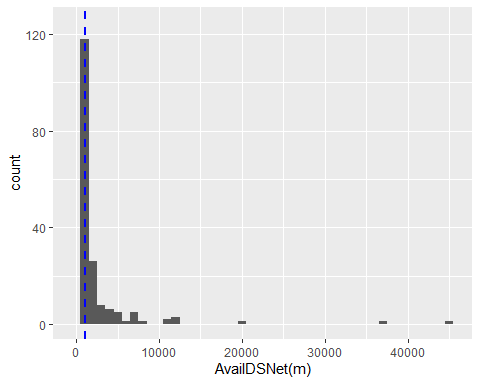
\includegraphics{EelHabitatMapMardown_files/figure-latex/unnamed-chunk-9-1.pdf}

\begin{verbatim}
## Warning: Removed 12 rows containing non-finite values (stat_bin).
\end{verbatim}

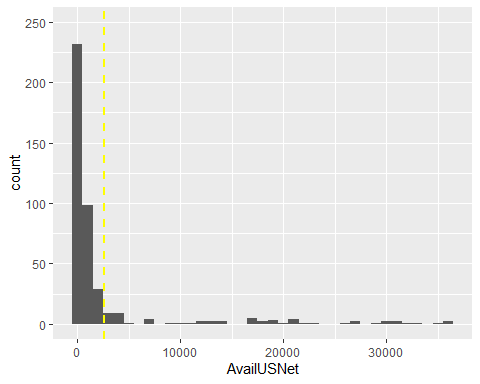
\includegraphics{EelHabitatMapMardown_files/figure-latex/unnamed-chunk-10-1.pdf}

{[}Range of habitat availability in upstream and downstream
directions{]}

The resulting habitat maps can be viewed on
\href{http://arcg.is/8qavW}{ArcGIS online}. Darker points show
structures that have the potential for releasing the most habitat
downstream or upstream if modified for fish passability. These layers do
not account for the quality of `available habitat' upstream/downstream.
`Habitat availability' is based on the assumption that all underlying
habitat is suitable for European Eel. In the absence of detailed
biological information or appropriate models of habitat quality this is
a common approach (see Buddendorf, 2017; Cote, 2009; Grill, 2014; Sheer,
2006). The layers also do not include information on the management of
individual structures. For example, a structure closed during Winter
Penn is likely to restrict access to all habitat downstream for eels
moving through the system. Somerset Wildlife Trust would like to include
information on the potential financial cost of improving structure
permeability in future iterations of the eel passability scores.

\hypertarget{discussion}{%
\section{Discussion}\label{discussion}}

\textless{}\textless{}\textless{}\textless{}\textless{}\textless{}\textless{}
HEAD

Culverts, tilting Weirs and Penstocks are the most frequently found
types of water control structures in the study area. Culverts create
problems with blockage of eel passage and interrupting gravel movement
(EA, 2010). Culverts are effectively large pipes used to connect bodies
of water together that are seperated by paths or roads. Depsite their
abundance in the Brue Valley area, due to the longitudinal profile of
European Eel culverts are not thought to present a major abstacle.
However, flap valves can be fitted to one culvert end to prevent the
back flow of water when pressure is greatest on the exit side of the
valve. Unless set open these flap valves should be judged as detrimental
to the passage of European Eel.

When prioritisng the installation of eel passes on tilting weirs, their
operation must must be assessed along with their structure (EA, 2010).
For example, a penning weir would only obstruct eel passage during
Winter months. Throughout spring and summer, it is flat. The migration
season (90\% of the run) for silver eels heading back to the coast
generally lasts from 1st August to 30th November (Sandlund \textbf{et
al}, 2017) and the IDB aims to achieve Winter levels in the Main Drain
by 1st December (see WLLMPs for South Drain and North Drain). Management
information was only available for 12\% (n=53) of water control
structures so the factor was not included in the barrier analsysis. This
information could be collected with local input from groundsmen at the
Environment Agency (pers comms, L. Timothy). The Internal Drainage Board
generally control smaller structure which require regular adjustment to
maintain water levels in local land areas over Winter and Summer seasons
(pers comms. P. Brewin). For these smaller more variable structures an
average height or position for the structure could be used.
\href{}{Comment}: More information is better than not enough

In-river structures such as penstocks generally fall into two
categories; undershot - where surplus water passes under the structure,
or overshot - where water weirs over a facet of the structure. Sometimes
a structure can be both overhsot and undershot.

The Eel Manual mentions `Available Habitat to next barrier' as a valid
priotisation strategy and was used to create the eel habitat map. The
Eels (England and Wales) Regulations 2009 Statutory Instrument (SI) came
into force on 15 January 2010 and supports Council Regulation (EC) No
1100/2007, which requires Member States to develop Eel Management Plans
(EMPs) for each river basin district, with the objective of permitting
the escapement to the sea of at least 40 \% of the historic silver eel
biomass. It was therefore essential that accepted criteria for barrier
prioritisation be developed, and a standard process, by which barriers
may be assessed and prioritised for eel passage and screening. Including
`Available Habitat to next barrier', a list of factors to be taken into
consideration when formulating a prioritisation strategy for eel passage
solutions is presented in the Eel Manual (EA, 2010); - Upstream
Productivity - Distance to next barrier - Available Habitat to next
barrier - Distance from head of tide - WFD status - Altitude -
Escapement potential - Passability - Structure Futures - Commercial
fishery operation - Parasitic status - Pesticide status - Silver eel
escapement compliance - Geographical location and spread - Designation
(SAC, SSSI) - Elver pass present - Ownership (EA) - Predator status -
Recreational benefit - Number of barriers below - Head drop -
Upstream/downstream eel population - Obstruction type - River Flow
conditions \& - Hydropower potential

\#Structure assessment surveys

A major issue identified by this map is the lack of individual
`permeability' or `passability' scores for each barrier. You need to
explain why these haven't been included yet in detail, provide
explanations for why you haven't used other tools and what your solution
is (ZSL eel assessment). Two or three examples of Species specific
connectivity software + studies to look at effect of barriers would be
good as well.

Individual passability scores for each barrier have not been included
due to a lack of data. Local stakeholders do not hold information on the
following aspects of water control structures needed for barrier
assessments; - Management, Management of structures has the greatest
effect on fish permeability. Piper (2013) found that management regimes
of sluice gate position, abstraction rate and weir spill strongly
affected probability of entrainment at intakes and the route choice of
eels. Management information was only available for a subset of the full
structure dataset. - Material - Aspect/Gradient These features cannot be
infered from satellite imagery and require surveys on the ground. There
are several protocols available for assessing the permeability of water
control structures to fish.

A more condensed list of factors for prioritisation on a catchment-based
approach has recently been presented by ZSL;

\begin{table}[t]

\caption{\label{tab:unnamed-chunk-11}Factors to consider when considering catchment level barrier prioritisation taken from 'A Field Guide for Assessing the Passability of Man-Made River Structures by European Eels}
\centering
\begin{tabular}{l|l|l}
\hline
  & Factors\_to\_Consider & Notes\\
\hline
1 & Structure overtopped at high tide & Structures that are overtopped during high tides can still be a high priority, if they do so infrequently\\
\hline
2 & Distance from the tidal limit & Highest priority to those impassable structures closest to the tidal limit\\
\hline
3 & Habitat availability upstream of barrier & Highest priority to those structures for which eel passage would open up larger amounts of upstream habitat\\
\hline
4 & Structures in close proximity upstream or downstream of the barrier & Lower priority to barriers with other impassable barriers upstream and/or downstream nearby, unless there are plans in the forseeable future to also put in eel passage facilities at those structures\\
\hline
5 & Alternative routes around the structure & Highest priority should be given to impassable structures for which alternative routes (channels) around the catchment do not exist\\
\hline
6 & Original purpose and current use of the structure & For example, consideration should be given if it is a gaiging weir\\
\hline
\end{tabular}
\end{table}

The factors presented within the Eel Manual or the ZSL field guide are
more easily formulatable into indices than those presented in the eel
manual. These indices can then be combined together in order to produce
a final passability score for individual structures. Installation of any
future eel passes on Environment Agency managed structures will most
likely only take place during capital works and refurbishments (pers
comms, M. Pang).

River regulation, in the form of damns or levees, restrict both the
lateral connectivity between the river and the floodplain and the
temporal and spatial variance in connectivity in the main stem of the
river (Ward \& Stanford, 1995; Kingsford, 2000). A number of GIS tools
and software packages exist for assessing the impact of water control
structures on river system connectivity.

\#The Vermont Culvert Aquatic Organism Passage Screening Tool

The Vermont Culvert Aquatic Organism Passage Screening Tool (Kirn2009)
consists of three components; the coarse screen, the retrofit potential
screen and habitat connectivity potential screen. The aquatic organism
passage coarse screen characterizes the expected level of aquatic
organism passage based on a set of physical measures of the culvert and
adjacent stream during low flow conditions. This first level of screen
is useful at the watershed and subwatershed scales to observe regional
conditions and to begin to identify structures having the most impact on
species of interest. The aquatic organism passage retrofit potential
screen identifies the likelihood of improving passage via structural
changes at a culvert. The aquatic organism passage habitat connectivity
potential screen indicates the amount of habitat that would be
re-connected if passage were to be improved at a structure (for example,
through installation of a fish pass). This screen is best applied at the
subwatershed and local catchment scales to realize the potential gains
in habitat due to changes at a specific structure or set of structures.

\hypertarget{sniffer}{%
\section{SNIFFER}\label{sniffer}}

\href{https://www.sniffer.org.uk/wfd111-phase-2a-fish-obstacles-manual-pdf}{The
WFD111 (2a) Coarse resolution rapid-assessment methodology to assess
obstacles to fish migration} (commonly known as the SNIFFER method) was
been developed to help prioritise the removal or mitigation of man-made
in-river structures that impede the migration of fish populations. It
has been designed to provide a procedure for rapidly assessing at a
coarse level the likely passability of obstacles. The methodology is
based on published data describing the swimming and leaping abilities of
different fish species. The method was tested against real fish
population data. SNIFFER has been used for minor assessments of natural
obstructions across Devon by the
\href{http://wrt.org.uk/sniffing-out-weirs/}{Westcountry Rivers Trust}
to moderate success (pers comms. S. West).

{[}WHo else has used SNIFFER?{]} {[}SNIFFER, 2011{]}{[}Bull{]}

{[}Why didn't you use it?{]}

\#FishXing

FishXing is a software designed to assist engineers, hydrologists and
fish biologists in the evaluation and design of culverts for fish
passage {[}FishXing2006{]} .The software requires the following inputs;
- Culvert Shape - Dimensions (diameter, rise, span) - Material and
Corrugation - Installation (At Grade or Embedded) - Culvert Length -
Culvert Slope (Can be automaticlally calculated if inlet and outlet
bottom elevations are known) - Culvert Outlet Bottom Elevation -
Entrance Loss (a constant used to determine the amount of energy loss as
the water enters the culvert inlet.) The software is only designed for
culverts which are frequenly installed in the United States under
highways are roads that bisect waterways. FishXing is still available
from the \href{https://www.fs.fed.us/biology/nsaec/fishxing/}{United
States Forest Service} as a Windows .exe build and provides
investigators an accurate indicator of a culvert's permeability to fish.
This could be useful tool for future work investigating movement within
SWT reserves. Once permeability scores have been gathered for water
control structures across the riverscape, connectivity models can be
used with GIS to develop prioritisation excercises.

\hypertarget{barrier-analysis-tool}{%
\section{Barrier Analysis Tool}\label{barrier-analysis-tool}}

The Barrier Analysis Tool (BAT) produced by the
\href{https://www.geodata.soton.ac.uk/geodata/gis/project173}{University
of Southampton} is a tool aiding managers in quantifying the amount of
river made available to fish through the removal of barriers would
provide valuable information in understanding the impact of barrier
removal and in evaluating the prioritisation of restoration actions. The
tool is available BAT is designed for the analysis of completely natural
systems and is unable to handle `loops' within the river network. Loops
are circular paths created when two polylines share the same to and from
nodes (see methodology for explanation of nodes). The Brue system
includes several heavily managed rivers which are important to
ecological flow not to mention the hundreds of dicthes that all create
loops within the river network line layer. Use of BAT was quickly
discounted on this basis.

\#FIPEX

=======

\hypertarget{a-major-issue-identified-by-this-map-is-the-lack-of-individual-permeability-or-passability-scores-for-each-barrier.-you-need-to-explain-why-these-havent-been-included-yet-in-great-detail-provide-explanations-for-why-you-havent-used-other-tools-and-what-your-solution-is-zsl-eel-assessment.-two-or-three-examples-of-species-specific-connectivity-software-studies-to-look-at-effect-of-barriers-would-be-good-as-well.}{%
\section{A major issue identified by this map is the lack of individual
`permeability' or `passability' scores for each barrier. You need to
explain why these haven't been included yet in great detail, provide
explanations for why you haven't used other tools and what your solution
is (ZSL eel assessment). Two or three examples of Species specific
connectivity software + studies to look at effect of barriers would be
good as
well.}\label{a-major-issue-identified-by-this-map-is-the-lack-of-individual-permeability-or-passability-scores-for-each-barrier.-you-need-to-explain-why-these-havent-been-included-yet-in-great-detail-provide-explanations-for-why-you-havent-used-other-tools-and-what-your-solution-is-zsl-eel-assessment.-two-or-three-examples-of-species-specific-connectivity-software-studies-to-look-at-effect-of-barriers-would-be-good-as-well.}}

Individual passability scores for each barrier have not been included
due to a lack of data. Local stakeholders do not hold information on the
following aspects of their water control structures; - Management,
Management of structures has the greatest effect on fish permeability.
{[}Piper2013{]} found that management regimes of sluice gate position,
abstraction rate and weir spill strongly affected probability of
entrainment at intakes and the route choice of eels. - Material -
Aspect/Gradient These features cannot be infered from satellite imagery
and require surveys on the ground. There are several protocols available
for assessing the permeability of water control structures to fish.

\hypertarget{national-inventory-and-assessment-procedurefor-identifying-barriers-to-aquatic-organism-passage-at-road-stream-crossings}{%
\section{NATIONAL INVENTORY AND ASSESSMENT PROCEDURE---For Identifying
Barriers to Aquatic Organism Passage at Road-Stream
Crossings}\label{national-inventory-and-assessment-procedurefor-identifying-barriers-to-aquatic-organism-passage-at-road-stream-crossings}}

\#The Vermont Culvert Aquatic Organism Passage Screening Tool
{[}Kirn2009{]} The Vermont Culvert Aquatic Organism Passage Screening
Tool consists of three components; the coarse screen, the retrofit
potential screen and habitat connectivity potential screen. The aquatic
organism passage coarse screen characterizes the expected level of
aquatic organism passage based on a set of physical measures of the
culvert and adjacent stream during low flow conditions. This first level
of screen is useful at the watershed and subwatershed scales to observe
regional conditions and to begin to identify structures having the most
impact on species of interest. The aquatic organism passage retrofit
potential screen identifies the likelihood of improving passage via
structural changes at a culvert. The aquatic organism passage habitat
connectivity potential screen indicates the amount of habitat that would
be re-connected if passage were to be improved at a structure (for
example, through installation of a fish pass). This screen is best
applied at the subwatershed and local catchment scales to realize the
potential gains in habitat due to changes at a specific structure or set
of structures.

\hypertarget{sniffer-1}{%
\section{SNIFFER}\label{sniffer-1}}

{[}What is SNIFFER{]} {[}How was it developed?{]} SNIFFER has been used
for minor assessments of natural obstructions across Devon by the
Westcountry Rivers Trust to moderate success (pers comms. S. West).

{[}SNIFFER, 2011{]}{[}Bull{]}

\#FIPEX

\begin{quote}
\begin{quote}
\begin{quote}
\begin{quote}
\begin{quote}
\begin{quote}
\begin{quote}
285b466eaaa74fa1a331da031f9b3b8ecc8d101f Where detailed and up-to-date
structure data other investigators have produced barrier permeability
models for other fish species over large scales. The Scottish barrier
prioritisation model was developed using the Fish Passage Extension
(FIPEX) for ArcGIS. FIPEX is able to produce a single comporable metric
of a structure's impact on fish passability known as the Dendretic
Connectivity Index (or DCI) which makes it useful for providing the
information necessary for local and national prioritisation of
management resources.
\end{quote}
\end{quote}
\end{quote}
\end{quote}
\end{quote}
\end{quote}
\end{quote}

Barrier prioritisation should be sensitive to habitat weighting since
not accounting for habitat quality can lead to over- or underestimating
the importance of impassable manmade barriers {[}@Buddendorf2018{]}.
{[}@Buddendorf2018{]} developed a flexible scalable approach for
assessing the effects of manmade barriers on longitudinal connectivity
for Atlantic salmon across Scotland, that considered the production
potential of different habitats, the potential effects of passable
manmade barriers under a range of passability values. The current
iteration of the map can be viewed
\href{http://marine.gov.scot/information/barriers-and-obstructions-freshwater-rivers}{here}

\begin{figure}
\centering
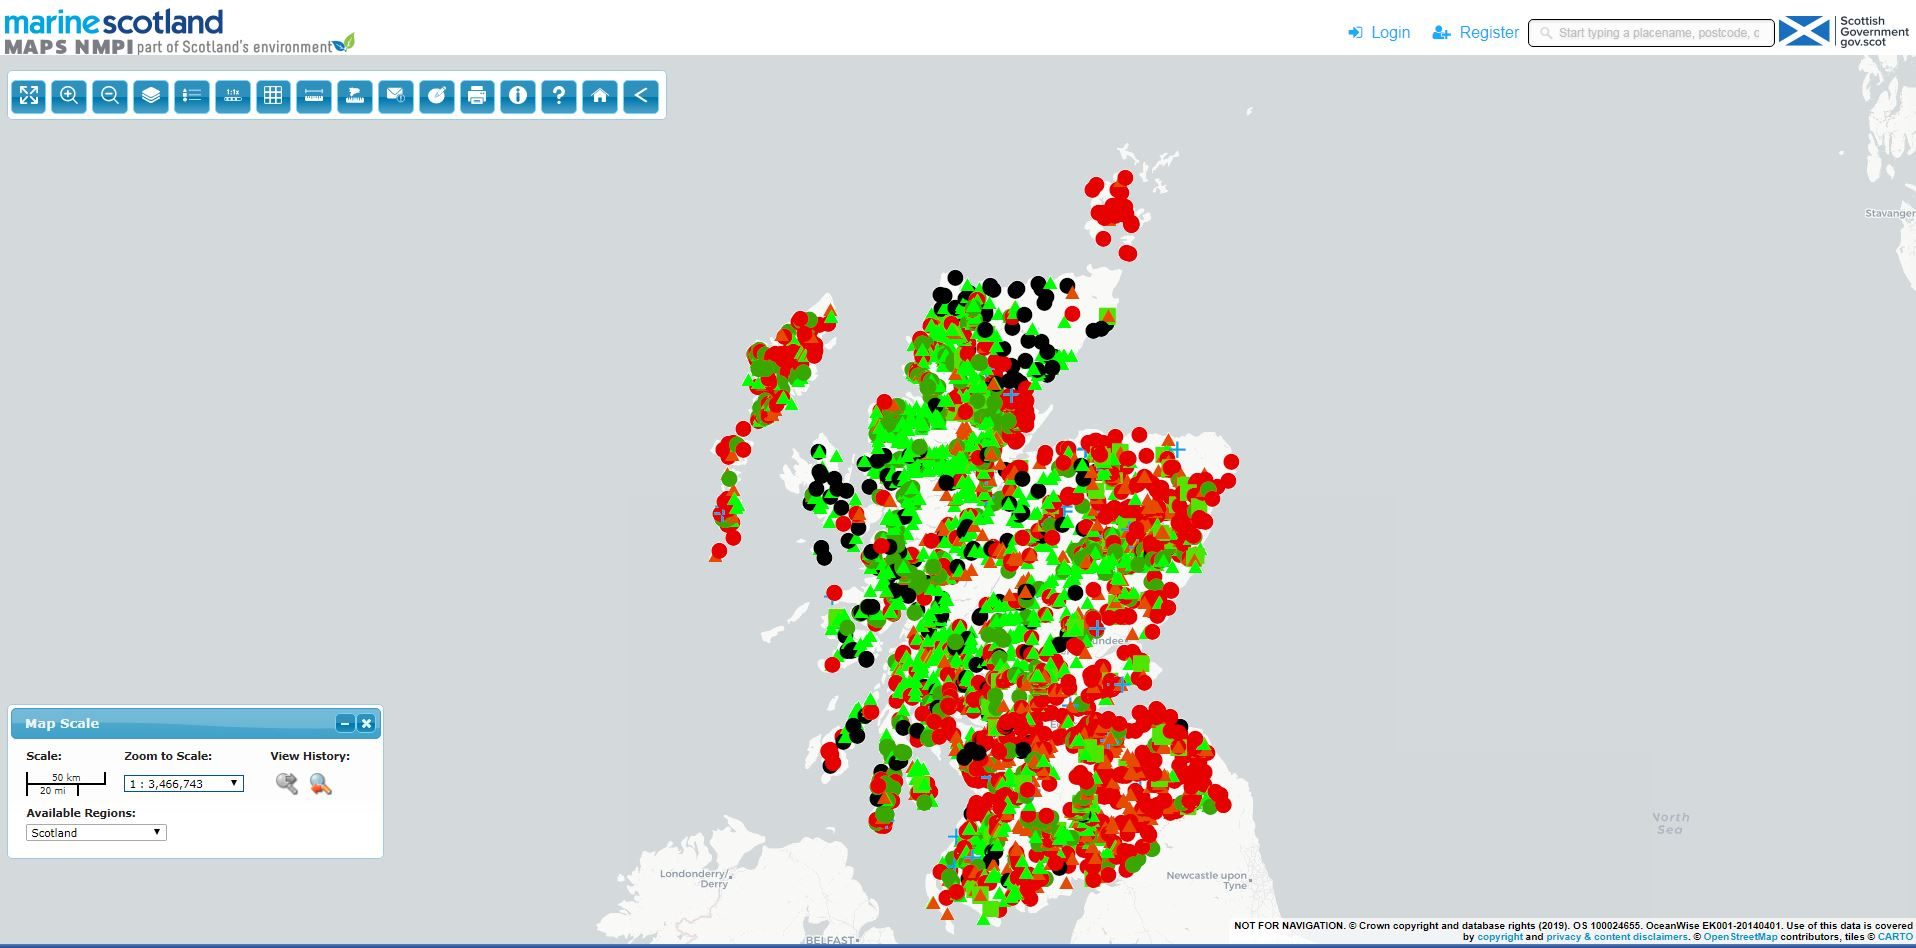
\includegraphics{Capture_ScotlandBarrierMap.jpg}
\caption{Alt text}
\end{figure}

The `passability' of barriers was informed by the
\href{https://www.sepa.org.uk/environment/environmental-data/}{Scottish
Obstacles to Fish Migration data set}. These data were initially
collated in the 1980s by staff from Marine Scotland Science using
information provided by District Salmon Fishery Boards, Fisheries Trusts
and local angling clubs. Additions were made to the map since the 80s
and a major update to the fish barrier dataset was produced in 2008
which is now managaed by the Scottish Environment Protection Agency.
{[}Buddendorf2018{]} developed their own metric for barrier passability
known as DCI\textsubscript{SCOT} which better accounted for the amount
of habitat available upstream as part of the barrier prioritisation
process {[}@Buddendorf2018{]}.
\textless{}\textless{}\textless{}\textless{}\textless{}\textless{}\textless{}
HEAD

Attempts were made to apply FIPEX to the Brue Valley Eel system however
the plug-in is no longer supported and doesn't function with ArcMap 10.6
{[}what year did this end? what version of ArcMap DOES it work with?{]}.
In order to make use of the underlying R code we also contacted the
authors of the Scottish barrier map. We were unable to obtain the
underlying R code for calculating DCI through data mining the original
plug-in or contacting FIPEX's authors {[}refer to FIPEX manual- why
doesn't the FIPEX manual come up in the mendeley search?{]}

{[}Mahlum2014a{]} demonstrated that the DCI produced by FIPEX shows
biological relevance with regards to understanding fish communities and
individual species distribution and abundance, even in the presence of
confounding variables such as elevation, stream width, and land cover.

For a more detailed review of connectivity modelling studies for
riverine systems please see {[}Fullerton2010{]}.

=======

Attempts were made to apply FIPEX to the Brue Valley Eel system however
the plug-is no longer supported and doesn't work with ArcMap 10.6
{[}what year did this end? what version of ArcMap DOES it work with?{]}.
In order to make use of the underlying R code we also contacted the
authors of the Scottish barrier map. We were unable to obtain the
underlying R code for calculating DCI through data mining the original
plug-in or contacting the FIPEX authors {[}refer to FIPEX manual- why
doesn't the FIPEX manual come up in the mendeley search?{]}

{[}Mahlum2014a{]} demonstrated that the DCI has biological relevance
with regards to understanding fish communities and individual species
distribution and abundance, even in the presence of confounding
variables such as elevation, stream width, and land cover.

\#FishXing
\textgreater{}\textgreater{}\textgreater{}\textgreater{}\textgreater{}\textgreater{}\textgreater{}
285b466eaaa74fa1a331da031f9b3b8ecc8d101f

FishXing is a software designed to assist engineers, hydrologists and
fish biologists in the evaluation and design of culverts for fish
passage {[}FishXing2006{]} .The software requires the following inputs;
- Culvert Shape - Dimensions (diameter, rise, span) - Material and
Corrugation - Installation (At Grade or Embedded) - Culvert Length -
Culvert Slope (Can be automaticlally calculated if inlet and outlet
bottom elevations are known) - Culvert Outlet Bottom Elevation -
Entrance Loss (a constant used to determine the amount of energy loss as
the water enters the culvert inlet.) The software is only designed for
culverts which are frequenly installed in the United States under
highways are roads that bisect waterways. FishXing is still available
from the \href{https://www.fs.fed.us/biology/nsaec/fishxing/}{United
States Forest Service} as a Windows .exe build and provides
investigators an accurate indicator of a culvert's permeability to fish.
This could be useful tool for future work investigating movement within
SWT reserves. For a more detailed review of connectivity modelling
studies for riverine systems please see {[}Fullerton2010{]}.

\hypertarget{recommendations}{%
\section{Recommendations}\label{recommendations}}

\begin{itemize}
\tightlist
\item
  Tables with top 3 passes for upstream, downstreamm and both
  directional movement
\item
  Future work to develop map further - add financial implications to
  decision making
\item
  Collect data from Environment Agency and IDB groundsmen on individual
  structure management
  \textless{}\textless{}\textless{}\textless{}\textless{}\textless{}\textless{}
  HEAD
\end{itemize}

\hypertarget{references}{%
\section{\# References}\label{references}}

\begin{quote}
\begin{quote}
\begin{quote}
\begin{quote}
\begin{quote}
\begin{quote}
\begin{quote}
285b466eaaa74fa1a331da031f9b3b8ecc8d101f
\end{quote}
\end{quote}
\end{quote}
\end{quote}
\end{quote}
\end{quote}
\end{quote}

Environment Agency Eel Manual, Eel and Elver Passes: Manual for the
Design and Implementation of Passage Solutioins, and Monitoring Eel and
Elver Populations Available from:
\url{https://www.gov.uk/government/publications/eel-and-elver-passes-design-and-build}

\hypertarget{appendices}{%
\section{Appendices}\label{appendices}}

\hypertarget{appendix-1---swt-gis-officer-feedback-on-draft-1.0---18.07.19}{%
\subsection{Appendix 1 - SWT GIS Officer feedback on Draft 1.0 -
18.07.19}\label{appendix-1---swt-gis-officer-feedback-on-draft-1.0---18.07.19}}

Hi Nathaniel,

Thanks for this, it's looking really good.

Data preparation

You say, Must not have gaps' and `Must not overlap' were set as the
topology rules. I'm Not sure what you mean here, `Must not have gaps'
isn't a topology rule that can be applied to lines?

Is it worth briefly describing what RivEX is?

Is it by design that the most of the ditches are not included in your
network?

Have you got permission from the IDB to publish the Rhyne and Structures
data on AGOL?

When I see these symbols on the map, the top and the bottom one look
very similar I would suggest making each one a distinct colour, e.g,
pink, red, blue etc and possibly make them a little larger.

Is there a way to show some examples of the potential habitat being
opened up by specific control structures visually on a map, e.g., if
control structure A is opened then all of these parts of the network
become available? Maybe using Service Areas in Network Analyst would
work? I would also be good to see further ways that this data could be
used as a practitioners tool. It would be awesome to have an interactive
tool whereby you can open and close control structures and see the
results on a map, this maybe a bit pie-in-sky though at the moment.

If think some of the attributes in the data tables need explaining,
e.g., all the US\_Accum2 attributes?

Thanks, Steve

Appendix 2 - Structure Surveys August 2019

A project for the Structure surveys was created within the EpiCollect5
data collection service to allow for data collection in the field using
the mobile application. Questions followed the ZSL `A Field Guide for
Assessing the Passability of Man-Made River Structures by European
Eels'.
\url{https://five.epicollect.net/project/brue-valley-structure-surveys}

The fourth question `Structure Name' should match the names (field = )
\url{http://arcg.is/1yCvHC}


\end{document}
